\section{Experimentação e resultados}

\begin{frame}{Experimentação e resultados}
    \begin{figure}[!htb]
        \centering
        
\includegraphics[scale=6]{images/test-tube}
    \end{figure}

\end{frame}


\begin{frame}{Ambiente de simulação - A rede Ipê}

    \begin{figure}[!htb]
        \centering
        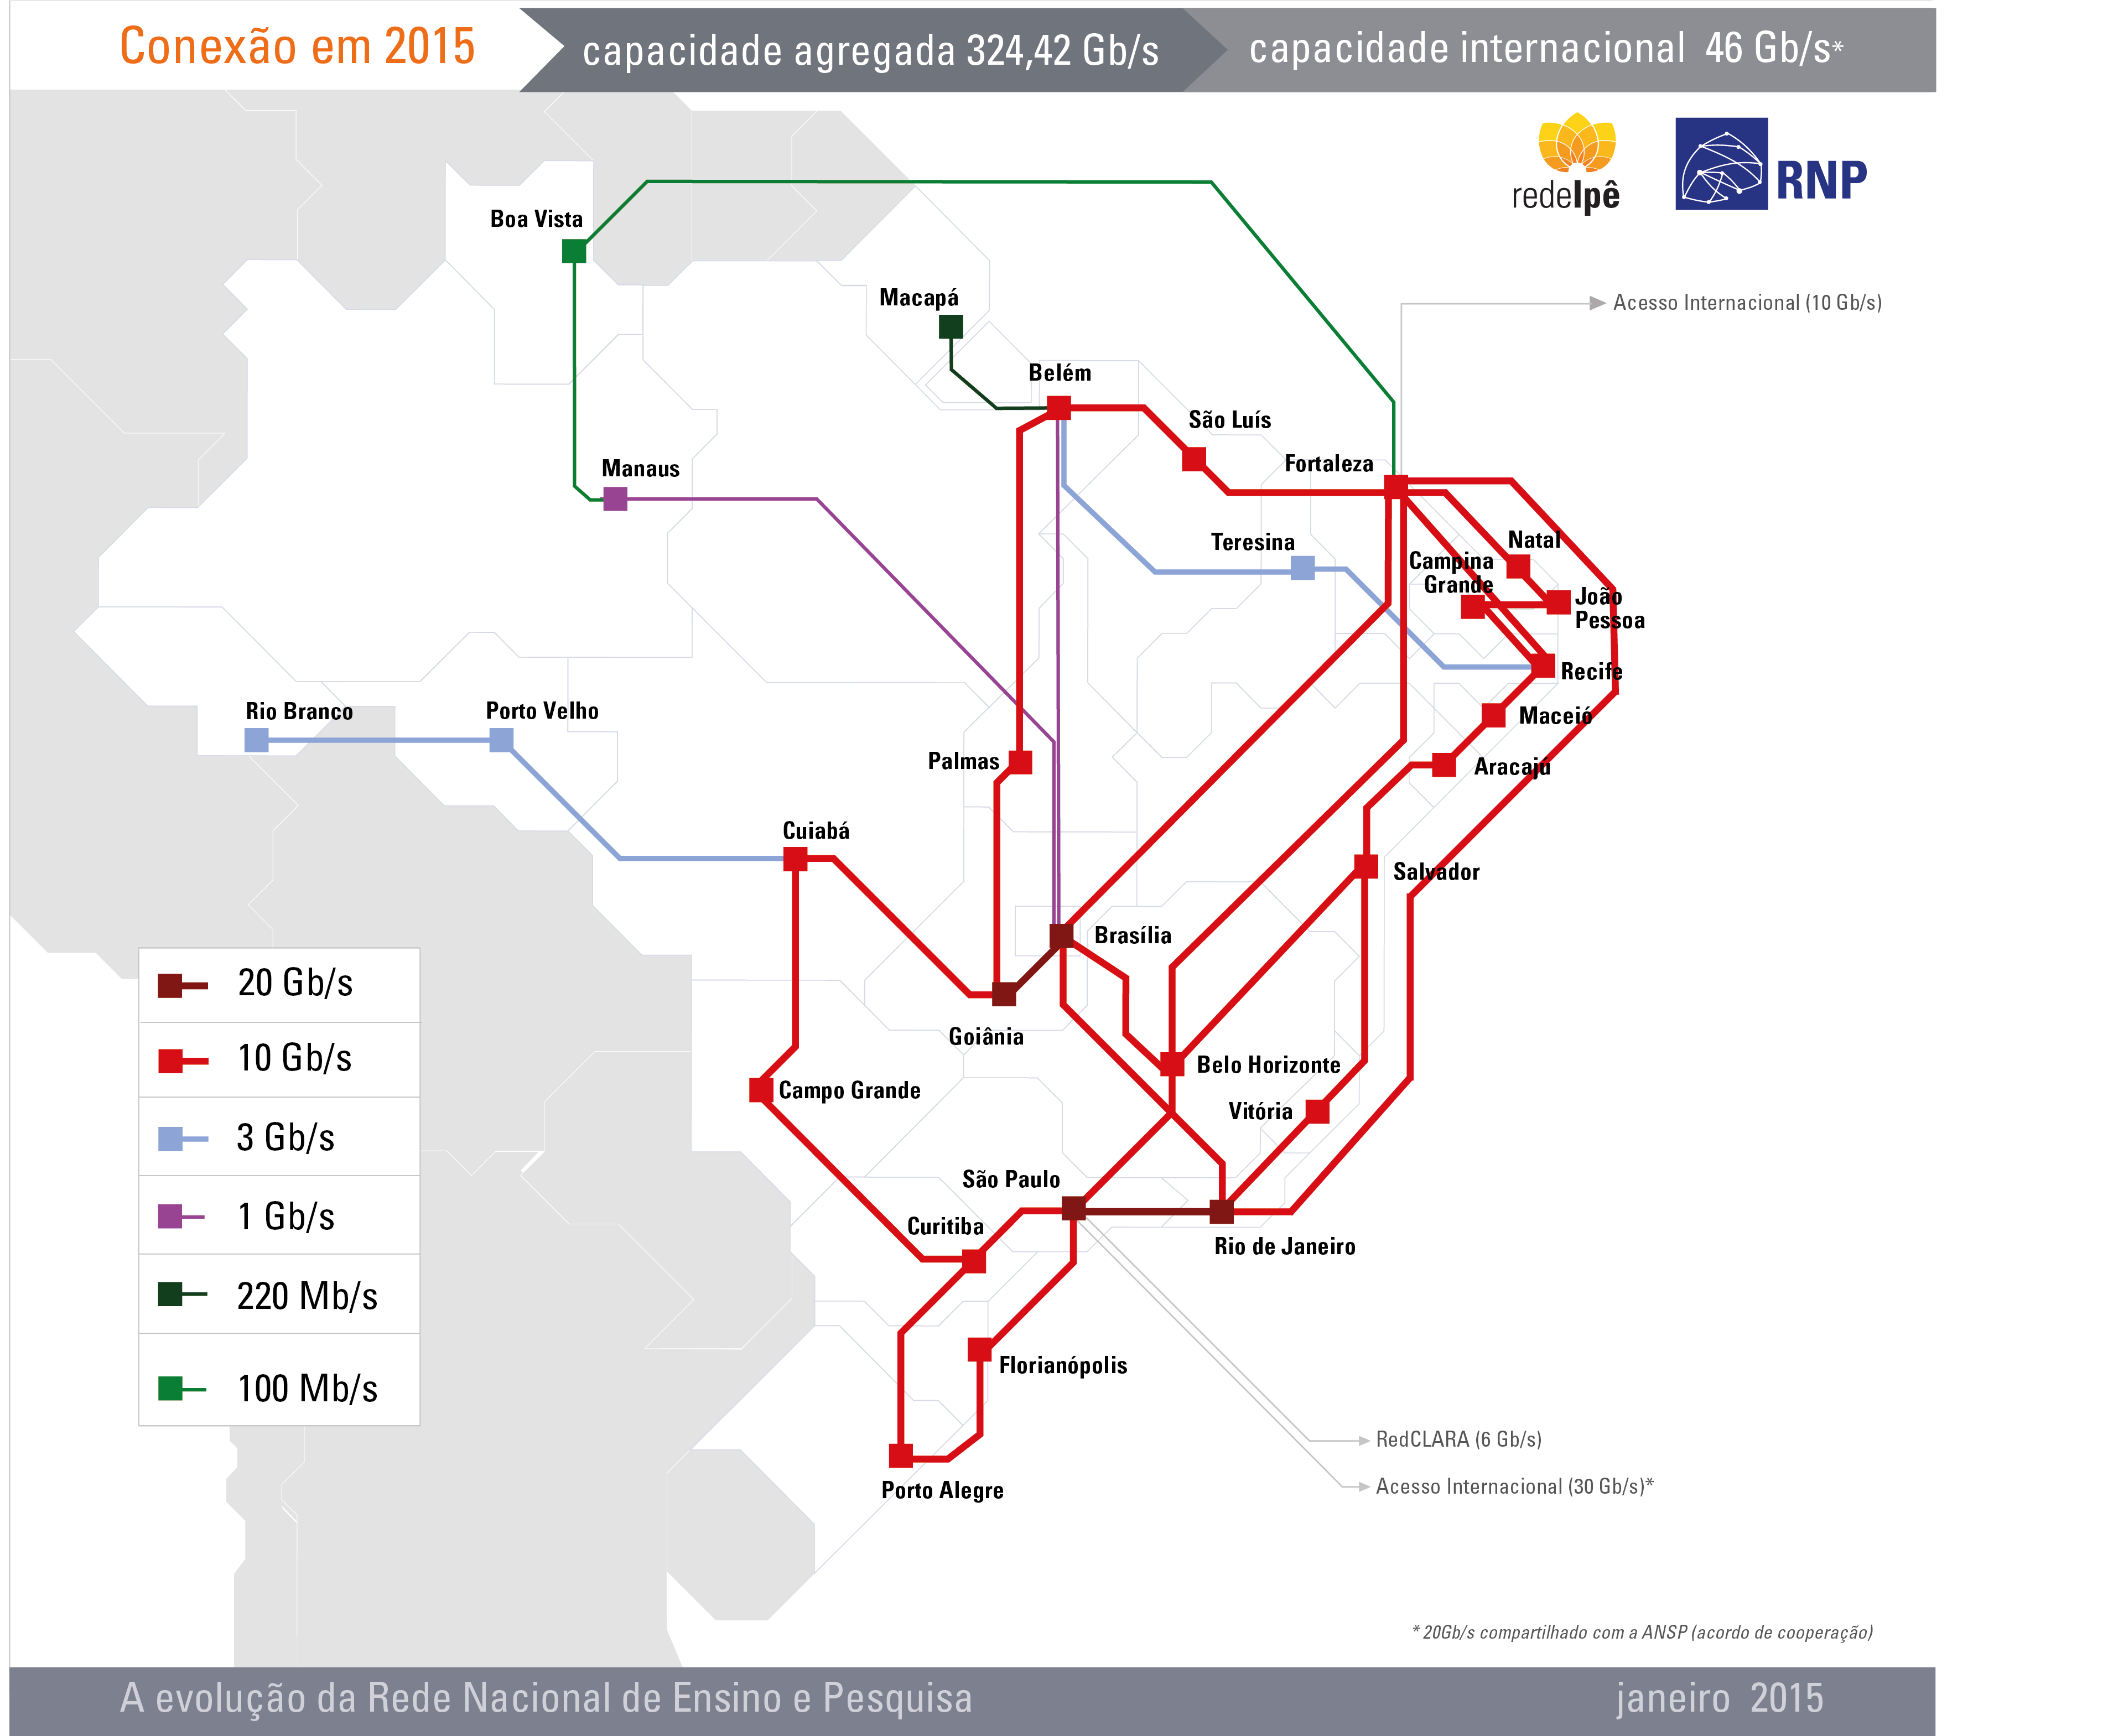
\includegraphics[scale=.15]{images/ipe-network-2015}
    \end{figure}

\end{frame}


\begin{frame}{Arquitetura da simulação}

    \begin{figure}[!htb]
        \centering
        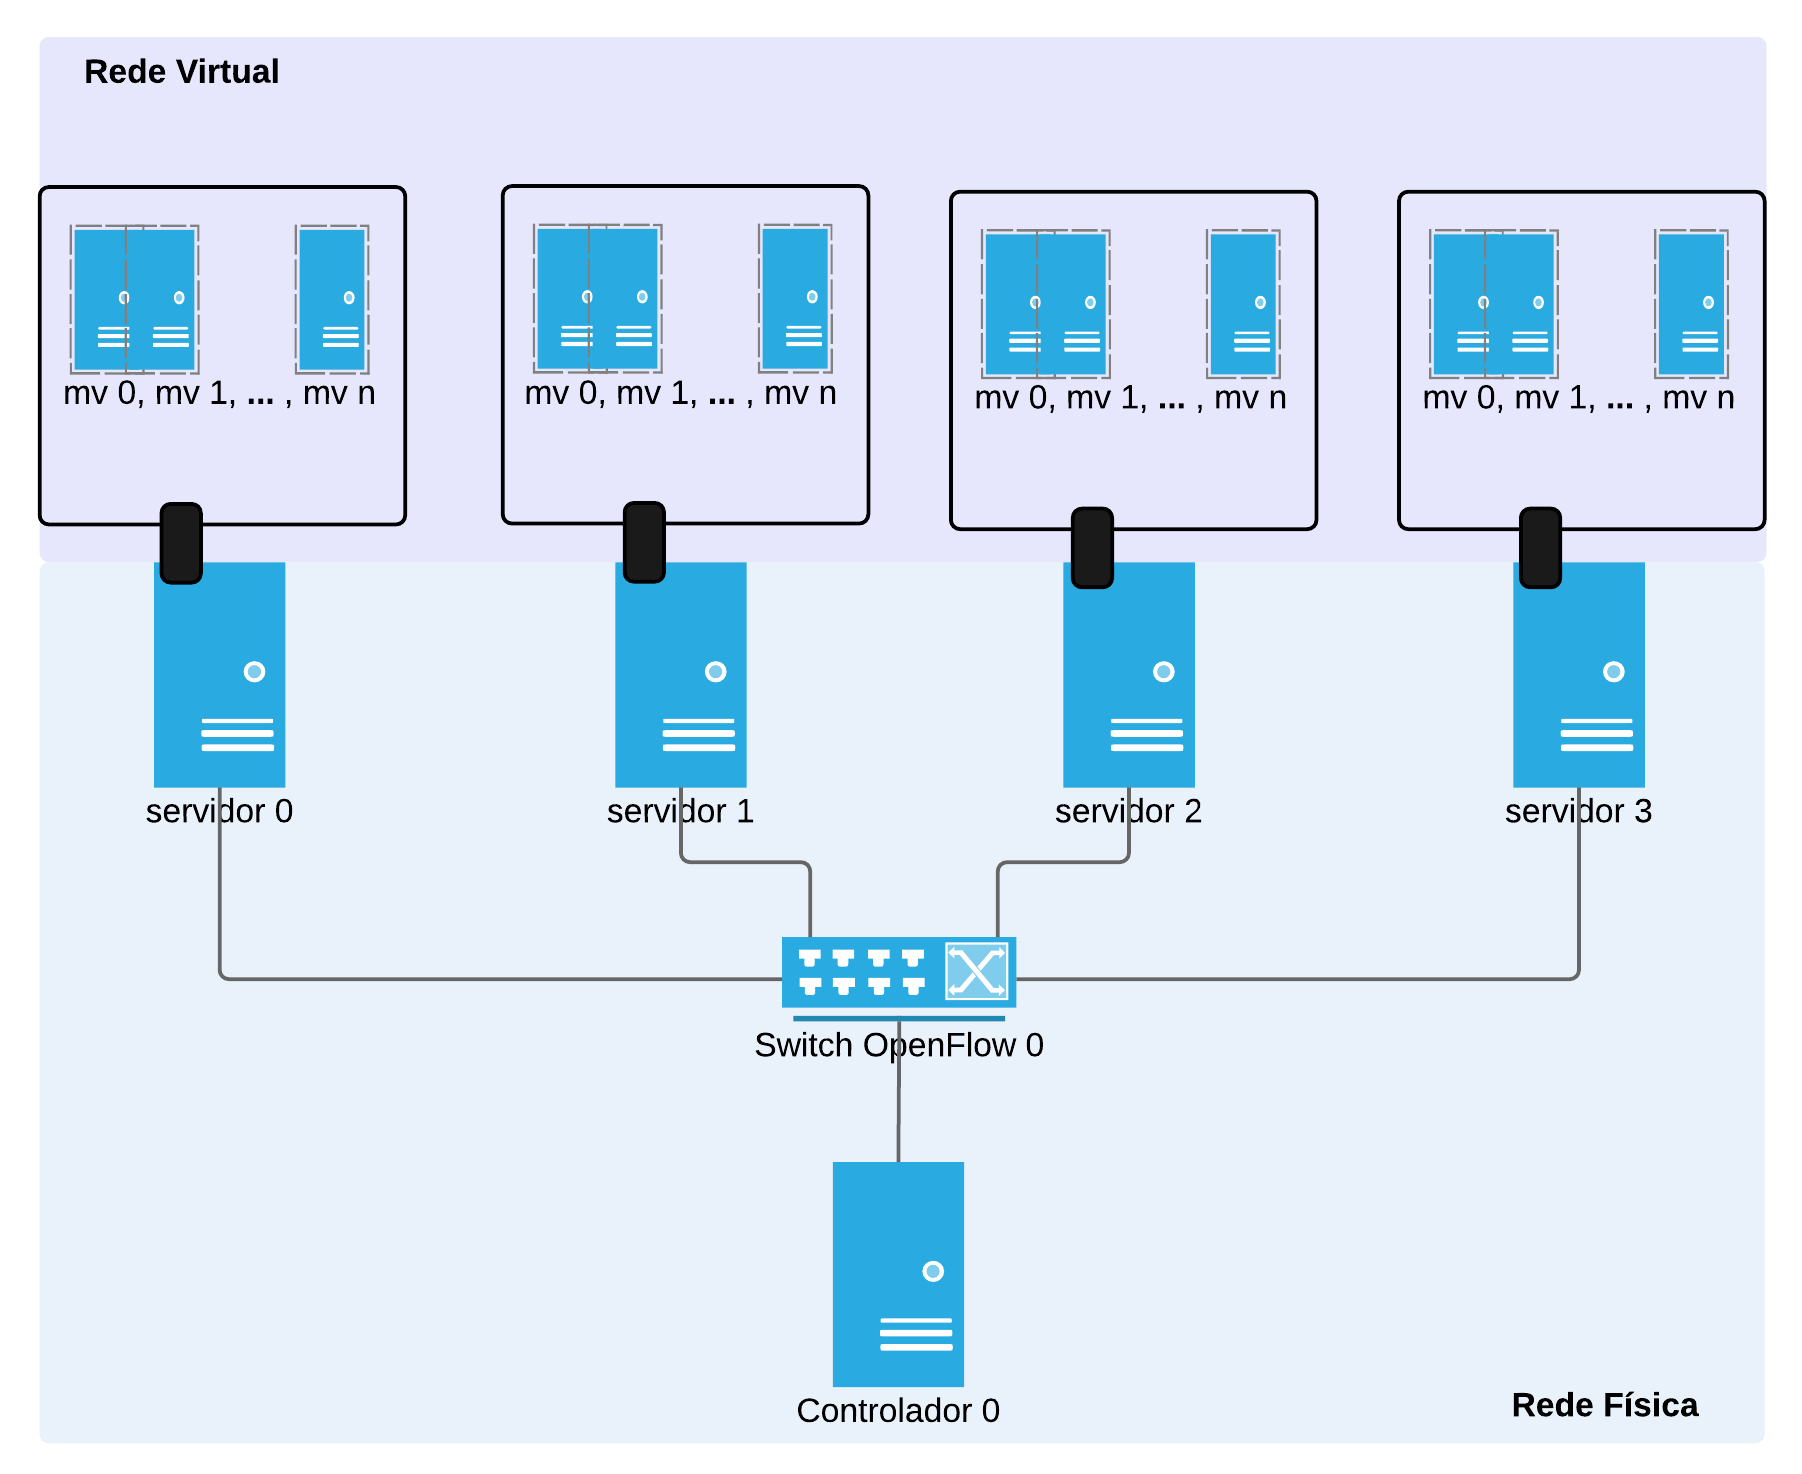
\includegraphics[scale=.55]{images/physical-vs-virtual-network-pt}
    \end{figure}

\end{frame}


\begin{frame}{Arquitetura da simulação}

    \begin{figure}[!htb]
        \centering
        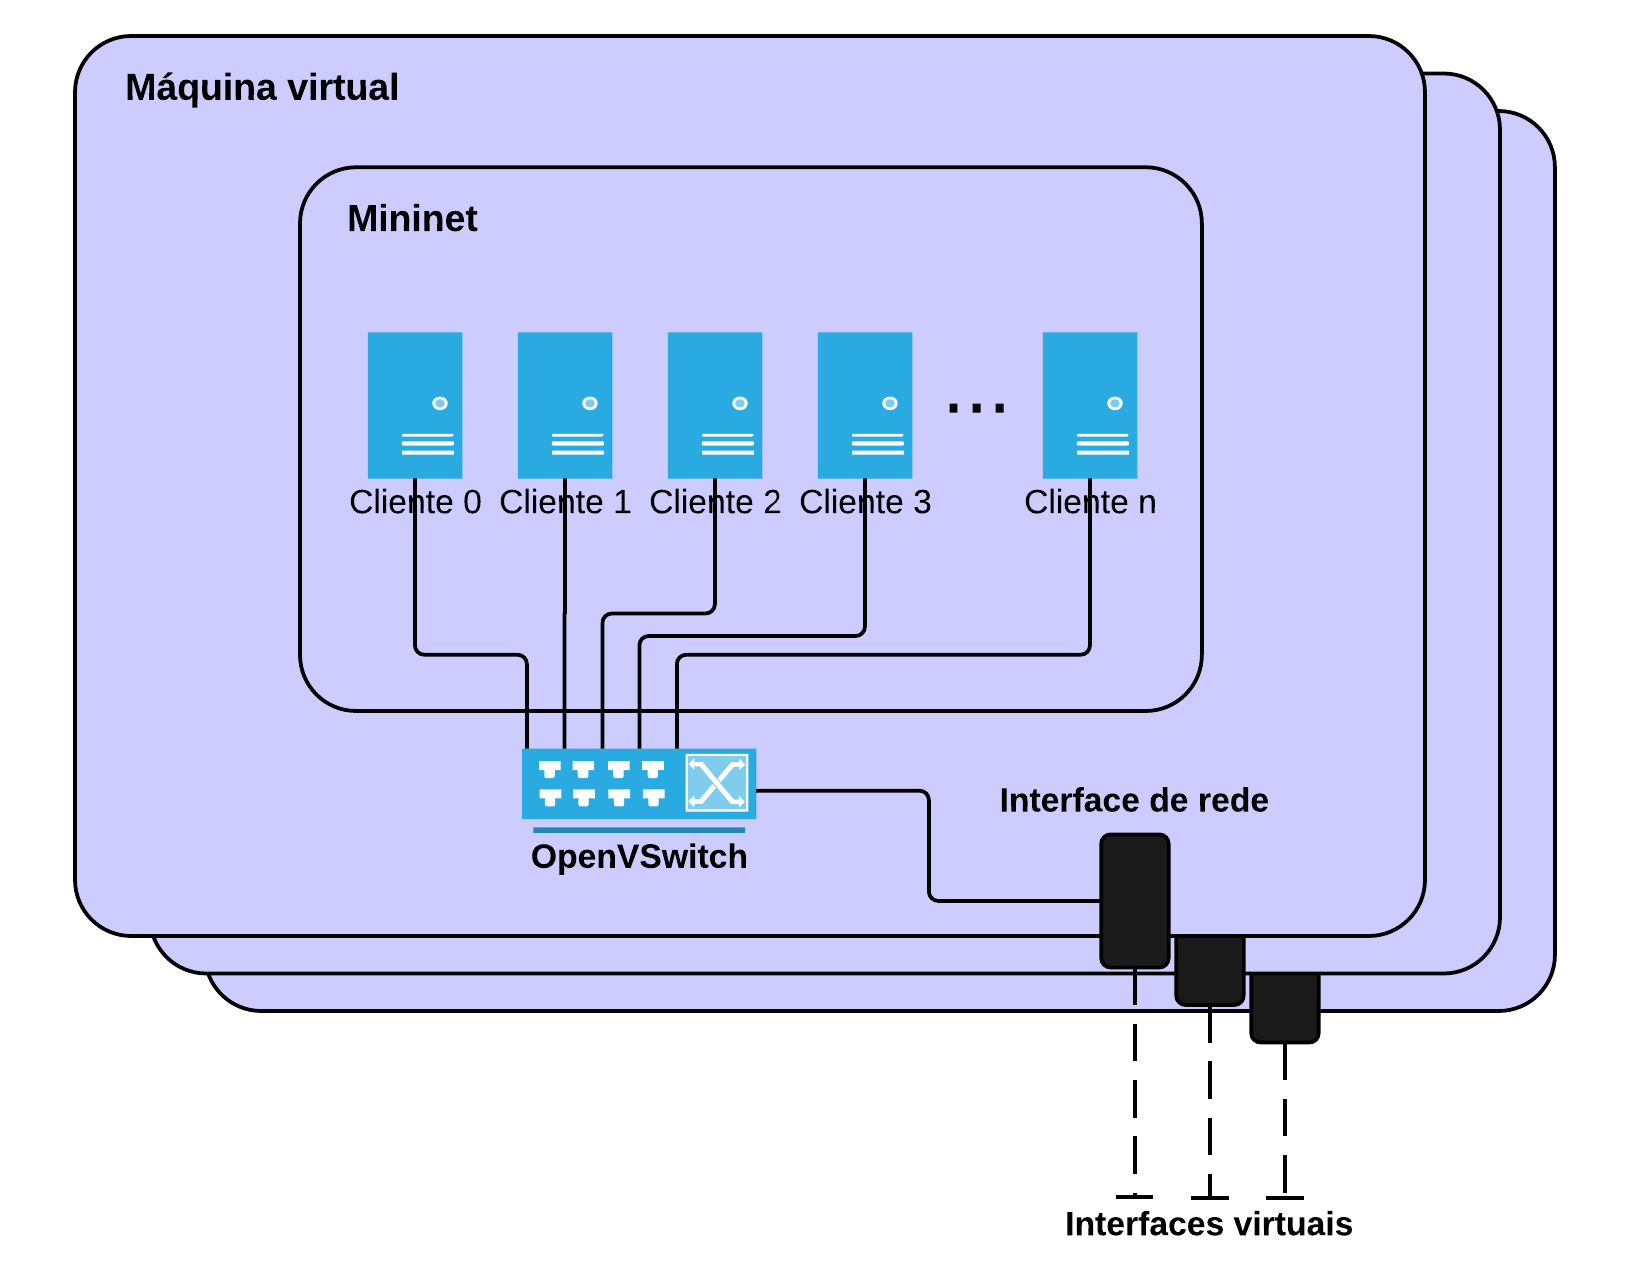
\includegraphics[scale=.55]{images/mininet-vm-architecture}
    \end{figure}

\end{frame}


\begin{frame}{Arquitetura da simulação}

    \begin{table}[h]
    \label{tbl:testbed-ipe-net}
    \centering
    \resizebox*{!}{\dimexpr\textheight- 25px}{
    \resizebox{\linewidth}{!}{
    \begin{tabular}{llllll}
        \rowcolor[HTML]{000000} 
        \multicolumn{6}{c}{\cellcolor[HTML]{000000}{\color[HTML]{C0C0C0} 
            \textbf{Associação de Servidores à simulação da rede IPÊ}}} \\
        \rowcolor[HTML]{000000} 
        {\color[HTML]{9B9B9B} \textbf{UF}} & {\color[HTML]{9B9B9B} 
            \textbf{N clientes}} & {\color[HTML]{9B9B9B} 
            \textbf{Sub-rede local}} & {\color[HTML]{9B9B9B} 
            \textbf{Servidor}} & {\color[HTML]{9B9B9B} \textbf{IP local}} & 
            {\color[HTML]{9B9B9B} \textbf{IP Gateway}} \\
        AC &  10 &  10.10.1.0 &   Shiva  &  10.10.42.51 & \\ 
        AL  & 13 &  10.10.2.0  &  Shiva  &  10.10.42.52 & \\ 
        AM  & 20 &  10.10.3.0 &   Shiva  &  10.10.42.53 & \\
        AP  & 7  &  10.10.4.0 &   Shiva  &  10.10.42.54 & 10.10.42.50 \\
        BA  & 25 &  10.10.5.0 &   Shiva  &  10.10.42.55 & \\
        CE  & 50  & 10.10.6.0  &  Shiva  &  10.10.42.56 & \\
        DF  & 16 &  10.10.7.0  &  Shiva  &  10.10.42.57 & \\ \hline
        ES  & 26  & 10.10.8.0  &  Eden  &   10.10.42.101 & \\
        GO  & 26  & 10.10.9.0  &  Eden  &   10.10.42.102  & \\  
        MA  & 7  &  10.10.10.0 &  Eden  &   10.10.42.103  & \\  
        MG  & 32  & 10.10.11.0  & Eden  &   10.10.42.104  & 10.10.42.100 \\  
        MS  & 10  & 10.10.12.0  & Eden  &   10.10.42.105  & \\  
        MT  & 8   & 10.10.13.0  & Eden  &   10.10.42.106  & \\  
        PA  & 13  & 10.10.14.0  & Eden  &   10.10.42.107  & \\ \hline
        PB  & 14  & 10.10.15.0  & Diablos & 10.10.42.151  & \\
        PE  & 41  & 10.10.16.0  & Diablos & 10.10.42.152  & \\  
        PI &  25 &  10.10.17.0 &  Diablos & 10.10.42.153  & \\  
        PR &  71 &  10.10.18.0 &  Diablos & 10.10.42.154  & 10.10.42.150 \\
        RJ &  27 &  10.10.19.0 &  Diablos & 10.10.42.155  & \\  
        RN &  11 &  10.10.20.0 &  Diablos & 10.10.42.156  & \\  
        RO &  10 &  10.10.21.0 &  Diablos & 10.10.42.157  & \\ \hline
        RR  & 7  &  10.10.22.0 &  Leviathan &   10.10.42.201 & \\
        RS &  10 &  10.10.23.0 &  Leviathan &   10.10.42.202  & \\  
        SC &  47 &  10.10.24.0 &  Leviathan &   10.10.42.203 & 10.10.42.200 \\   
        SE &  13 &  10.10.25.0 &  Leviathan &   10.10.42.204 & \\   
        SP &  25 &  10.10.26.0 &  Leviathan &   10.10.42.205  & \\  
        TO &  11 &  10.10.27.0 &  Leviathan &   10.10.42.206 & \\   
    \end{tabular}
    }}
\end{table}

\end{frame}


\begin{frame}[fragile]{Detecção de entidades}

\begin{lstlisting}[ tabsize=4,  
                    language=bash,
                    basicstyle=\ttfamily\footnotesize,
                    aboveskip={1.5\baselineskip},
                    columns=fixed,
                    showstringspaces=false,
                    extendedchars=true,
                    breaklines=true,
                    frame=single,
                    numbers=left,
                    showtabs=false,
                    showspaces=false,
                    showstringspaces=false,
                    identifierstyle=\ttfamily,
                    ]
INFO:topology.graph:SwitchJoin id: 2
INFO:topology.graph:SwitchJoin id: 1
INFO:topology.graph:1, 2
DEBUG:openflow.discovery:Dropping LLDP packet 275
INFO:topology.graph:LinkEvent fired
INFO:host_tracker:Learned 1 1 7e:e6:9b:89:39:2e got IP 10.0.0.1
INFO:topology.graph:HostJoin id: 7e:e6:9b:89:39:2e
INFO:host_tracker:Learned 2 1 62:77:44:24:13:49 got IP 10.0.0.2
INFO:topology.graph:HostJoin id: 62:77:44:24:13:49
\end{lstlisting}

\end{frame}


\begin{frame}{Remoção de computadores}

    \begin{figure}[!htb]
        \centering
        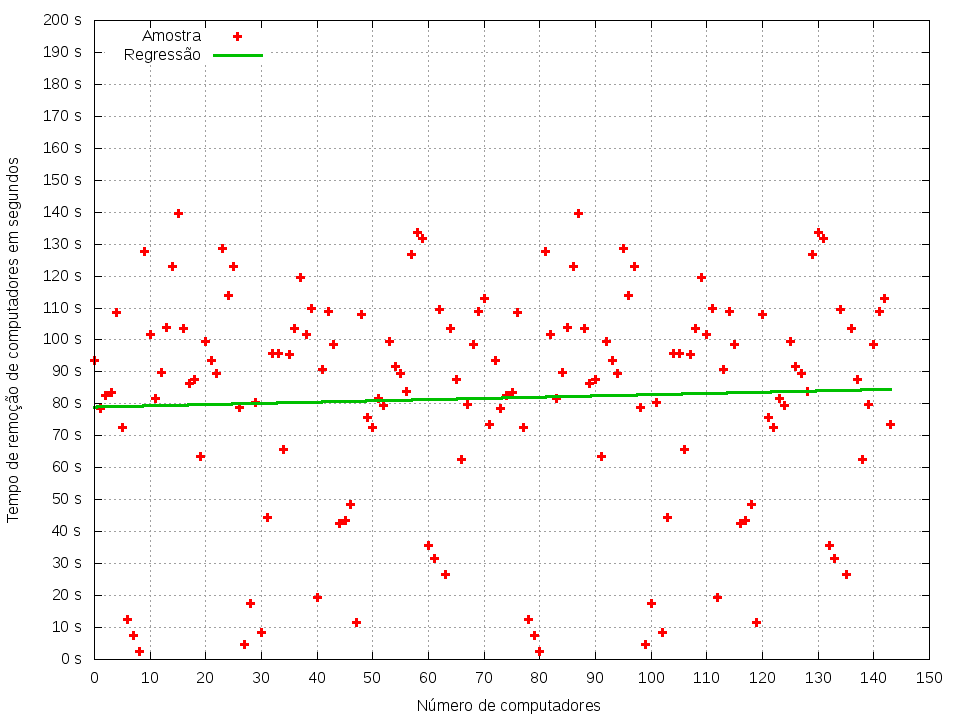
\includegraphics[scale=.35]{images/hosts-leave-time}
    \end{figure}

\end{frame}


\begin{frame}{Remoção de \emph{switches}}

    \begin{figure}[!htb]
        \centering
        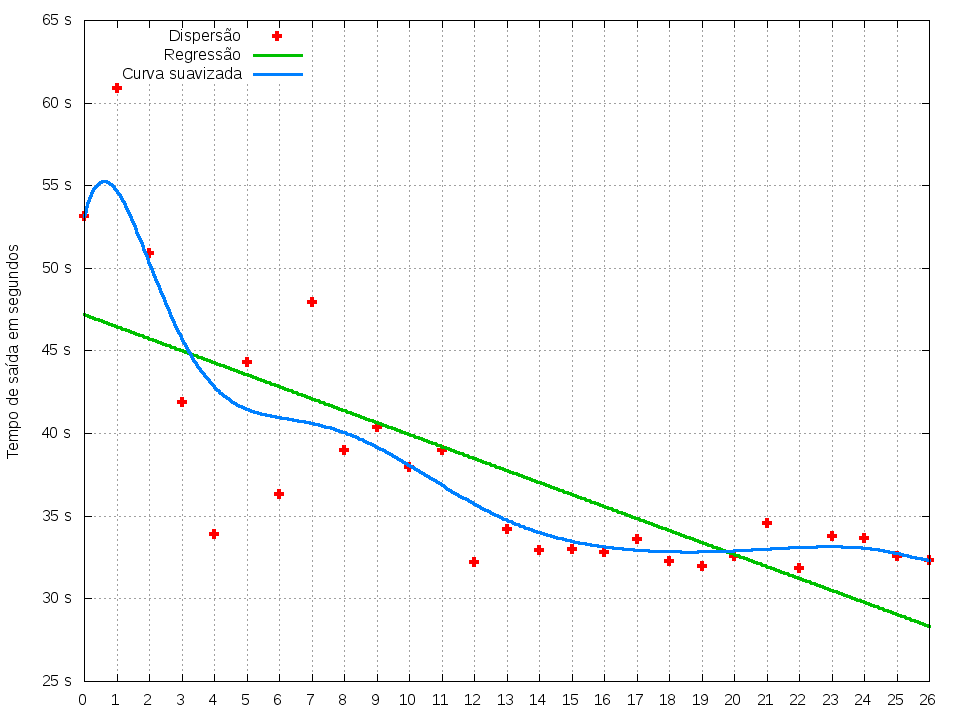
\includegraphics[scale=.35]{images/switch-leave-time}
    \end{figure}
\end{frame}


\begin{frame}{Remoção de computadores por \emph{switch}}

    \begin{figure}[!htb]
        \centering
        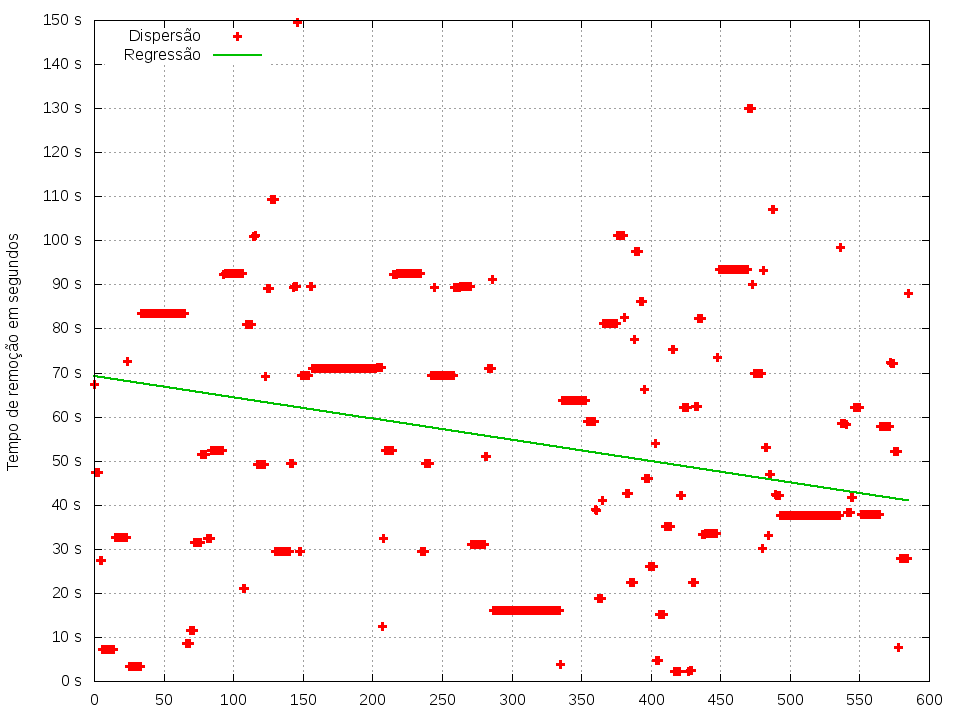
\includegraphics[scale=.35]{images/hosts-behind-switch-time}
    \end{figure}
\end{frame}


\begin{frame}{Visualização em tempo real}

    \begin{figure}[!htb]
        \centering
        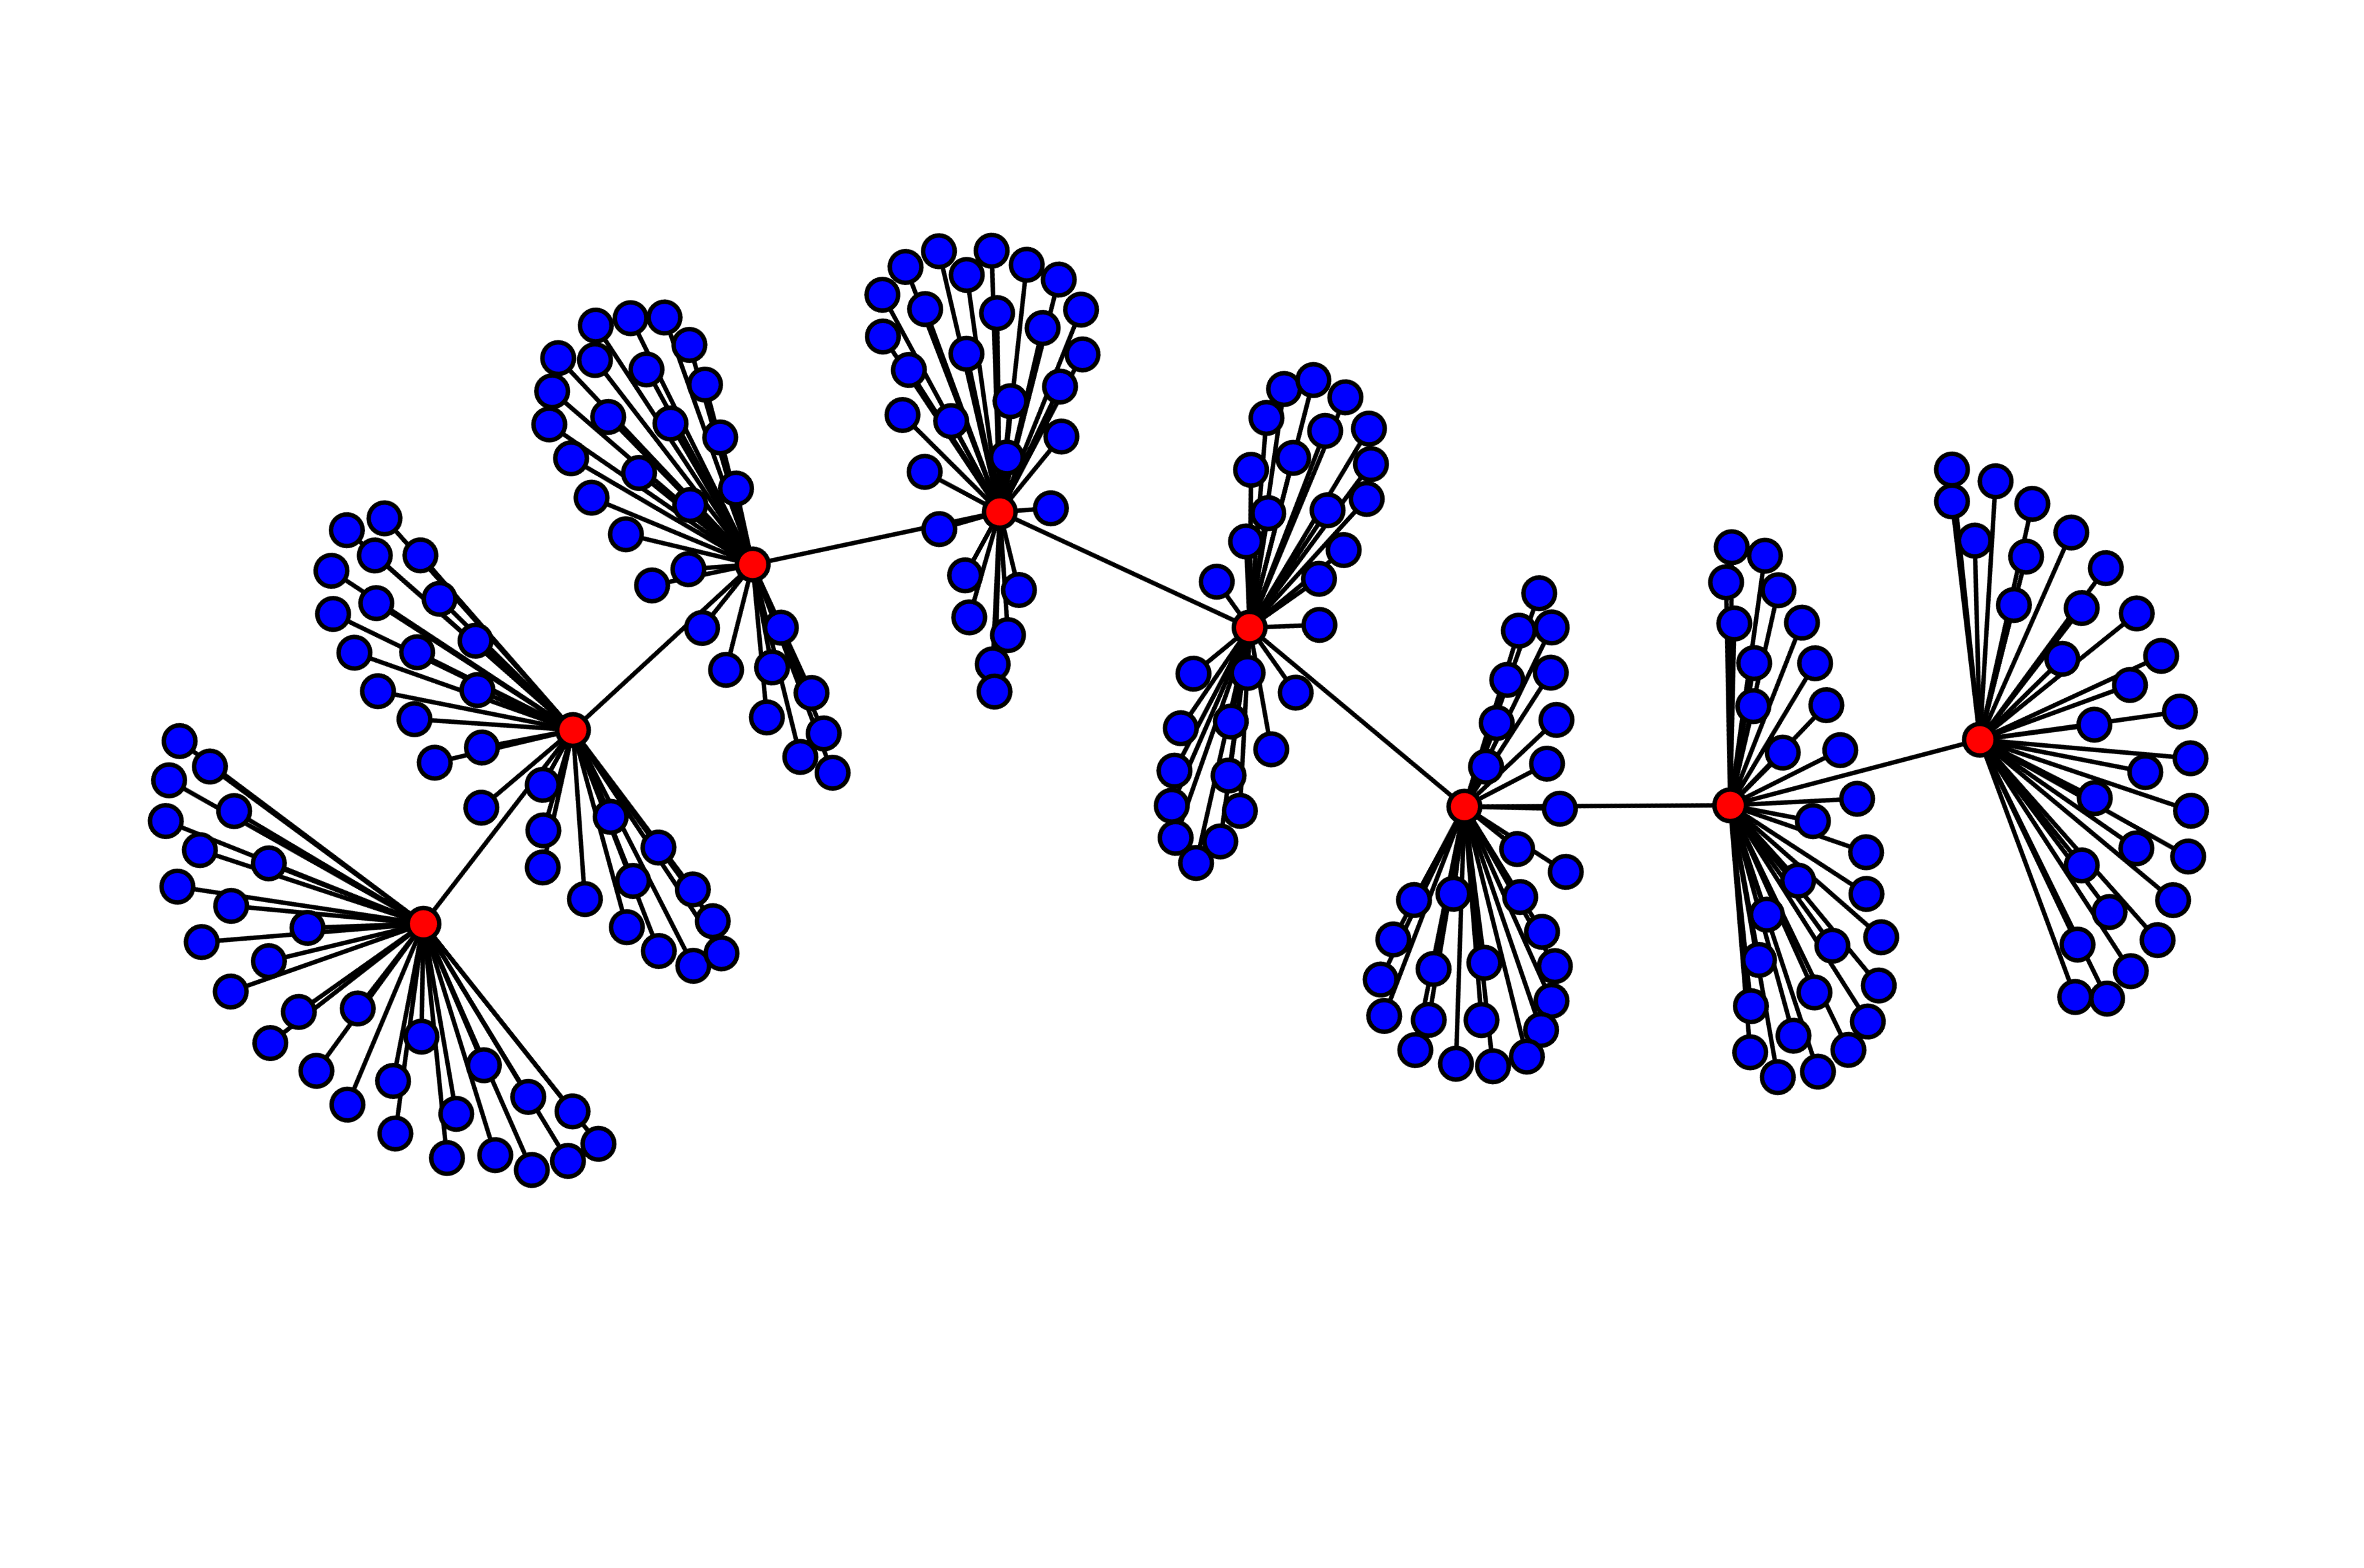
\includegraphics[scale=.6]{images/full-graph}
    \end{figure}
\end{frame}


\begin{frame}{Visualização em tempo real}

    \begin{figure}[!htb]
        \centering
        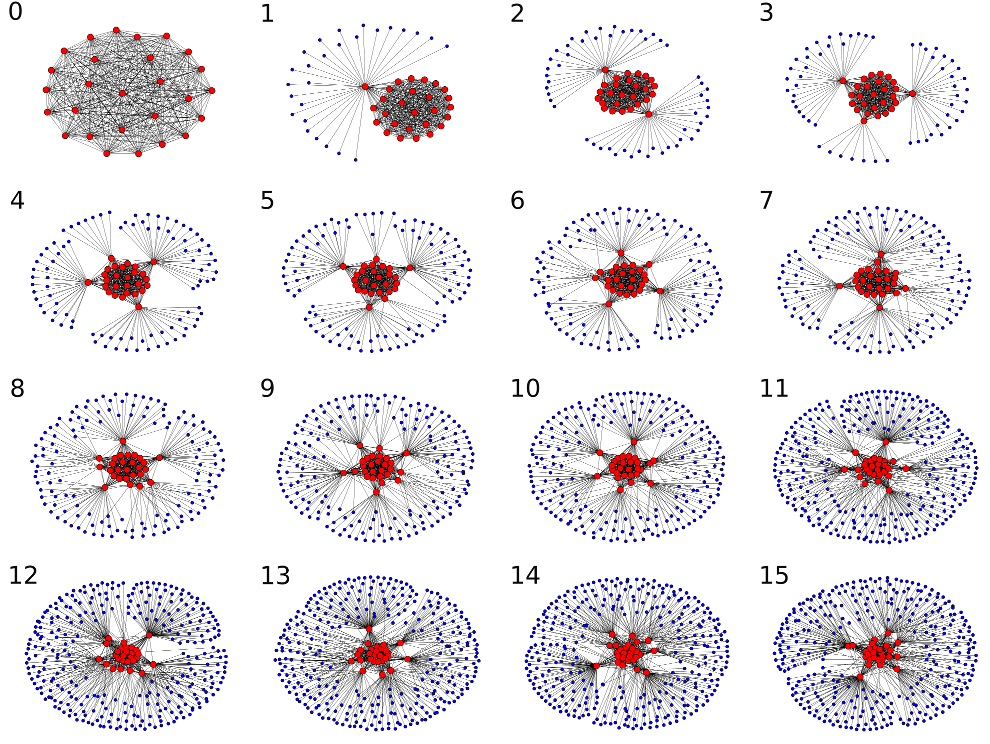
\includegraphics[scale=.25]{images/full-graph-ipe-0}
    \end{figure}
\end{frame}

\begin{frame}{Visualização em tempo real}

    \begin{figure}[!htb]
        \centering
        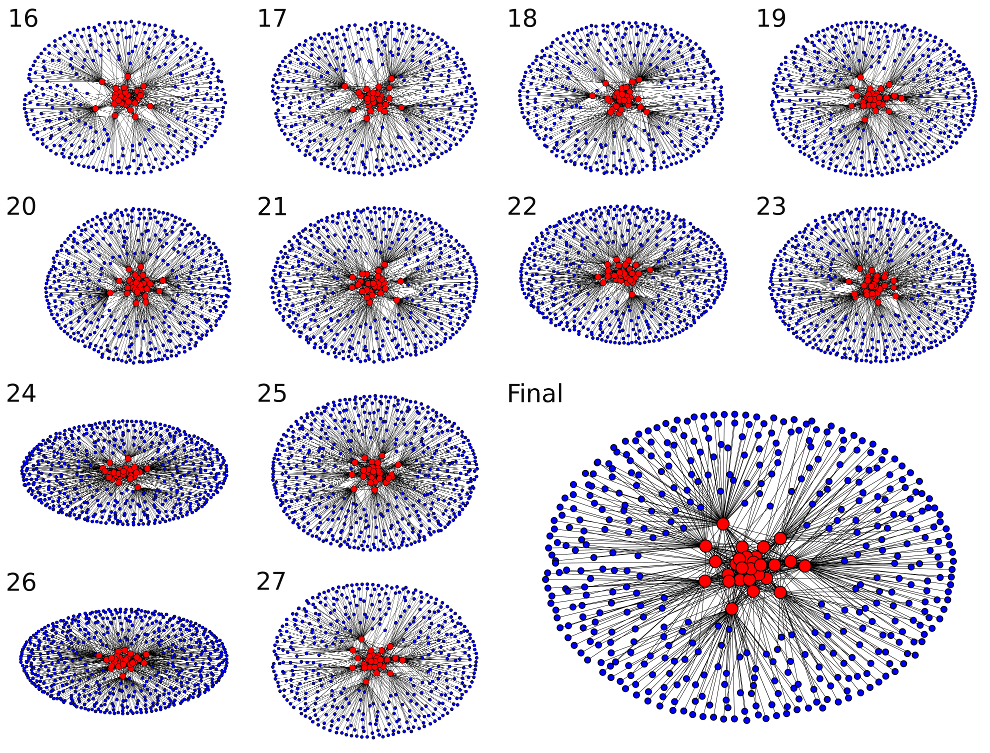
\includegraphics[scale=.25]{images/full-graph-ipe-1}
    \end{figure}
\end{frame}


\begin{frame}{Identificação de tráfego na rede}

    \begin{figure}[!htb]
        \centering
        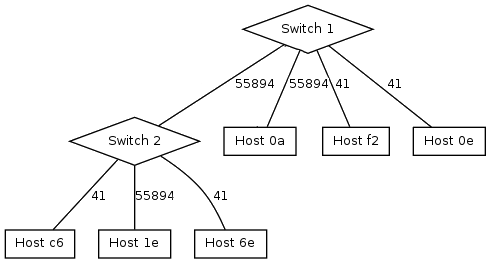
\includegraphics[scale=.6]{images/graph-iperf}
    \end{figure}
\end{frame}



\begin{frame}{Consumo de processador no controlador}

    \begin{figure}[!htb]
        \centering
        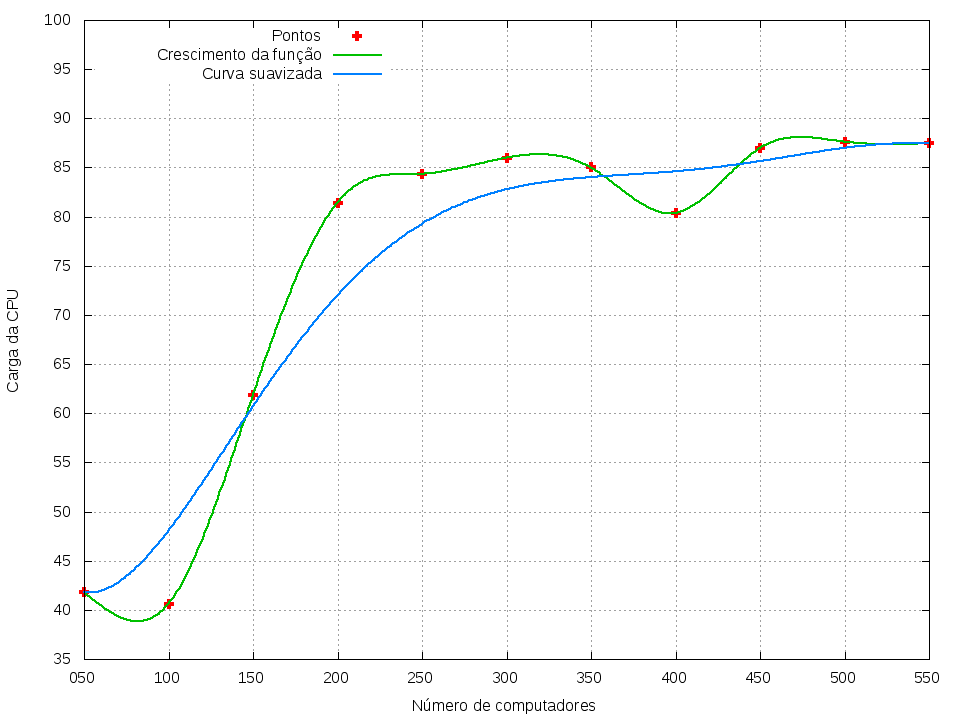
\includegraphics[scale=.35]{images/usr-cpu-growth}
    \end{figure}
\end{frame}


\begin{frame}{Consumo de processador no controlador}

    \begin{figure}[!htb]
        \centering
        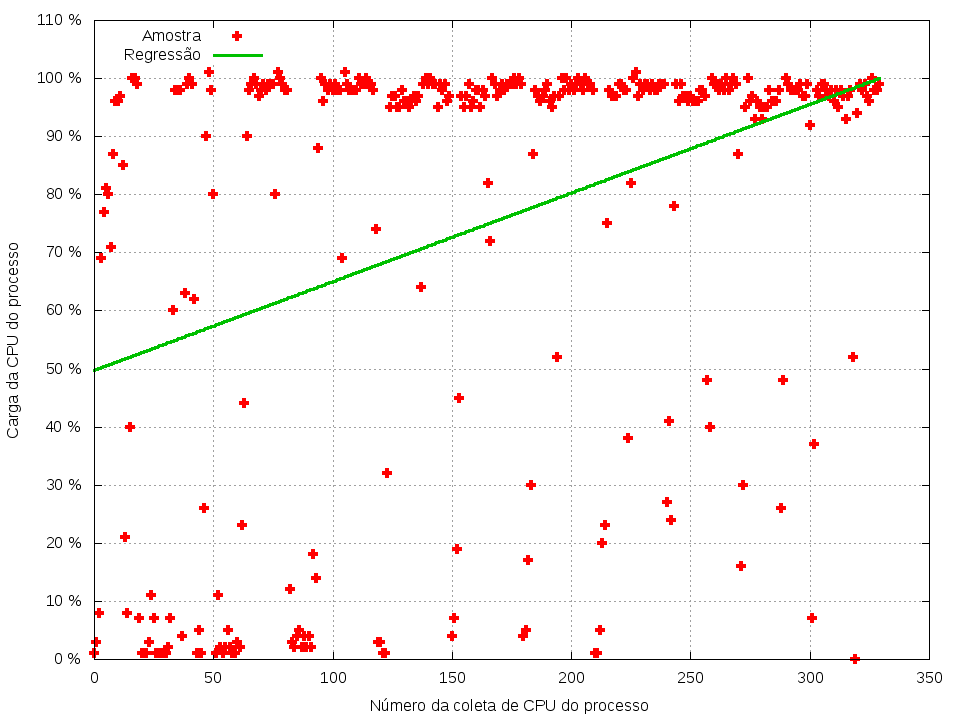
\includegraphics[scale=.35]{images/scatter-usr-cpu}
    \end{figure}
\end{frame}



\begin{frame}{Consumo de processador em relação ao SO}

    \begin{figure}[!htb]
        \centering
        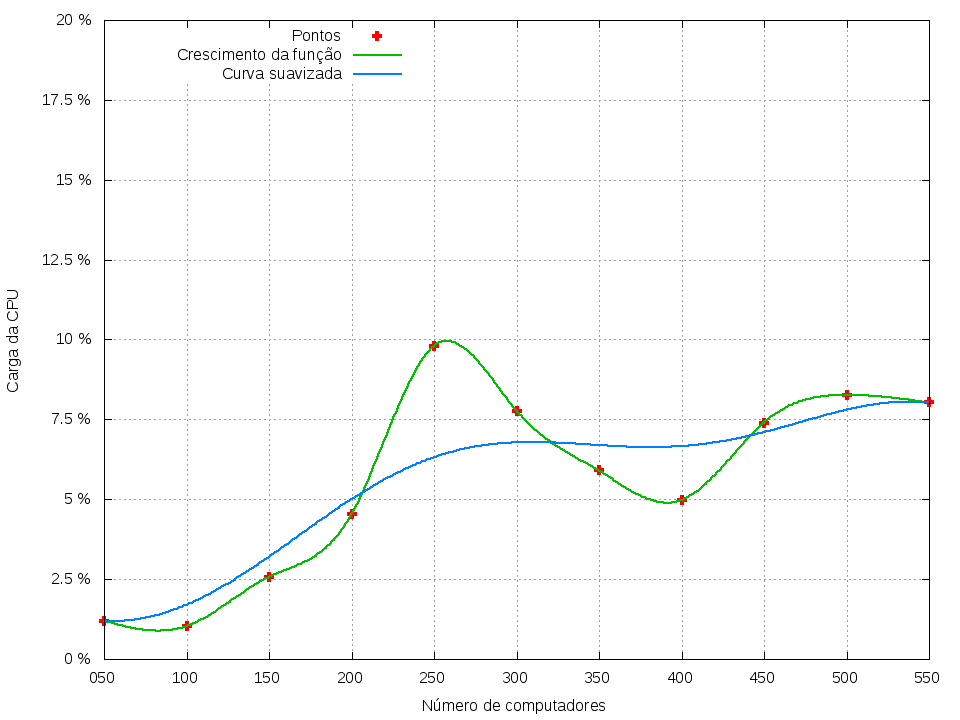
\includegraphics[scale=.35]{images/sys-cpu-growth}
    \end{figure}
\end{frame}



\begin{frame}{Consumo de processador em relação ao SO}

    \begin{figure}[!htb]
        \centering
        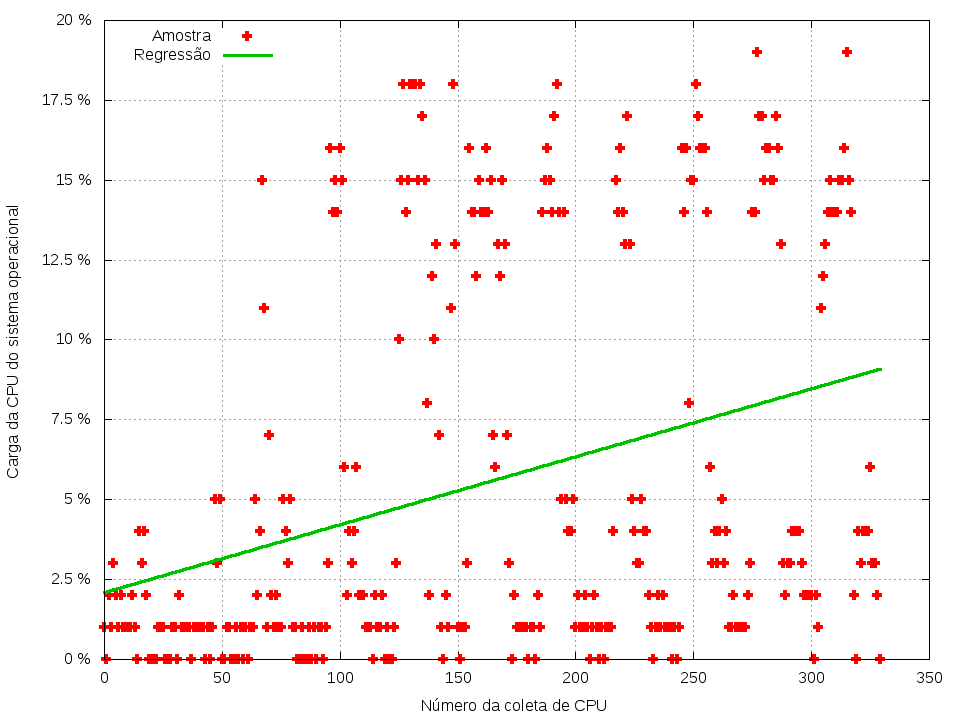
\includegraphics[scale=.35]{images/scatter-sys-cpu}
    \end{figure}
\end{frame}


\begin{frame}{Consumo de memória}

    \begin{figure}[!htb]
        \centering
        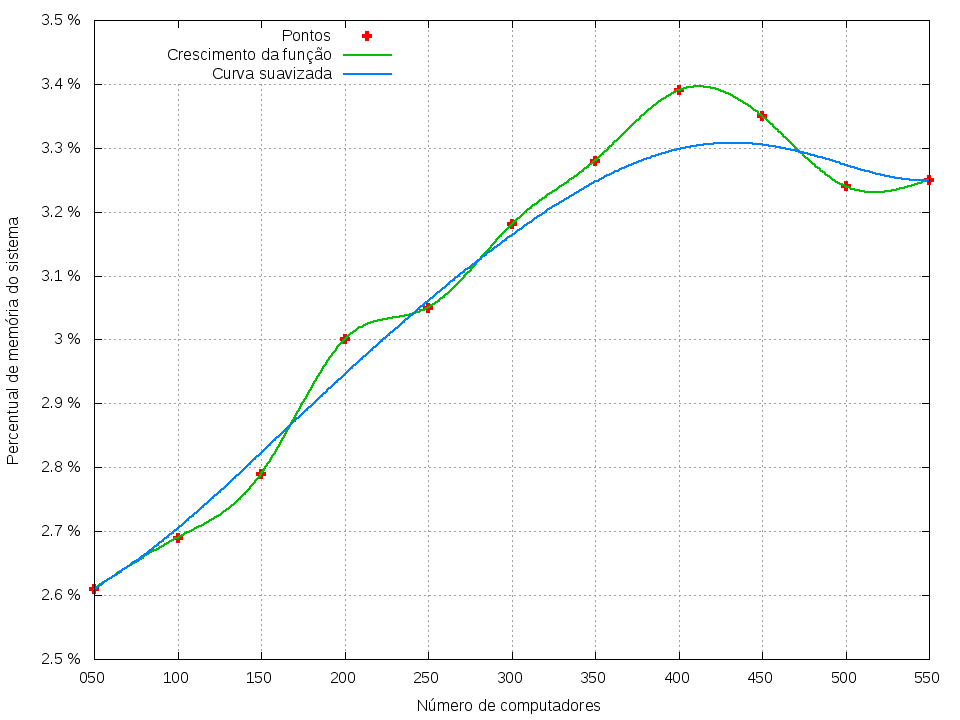
\includegraphics[scale=.35]{images/memory-usage-growth}
    \end{figure}
\end{frame}



\begin{frame}{Consumo de memória}

    \begin{figure}[!htb]
        \centering
        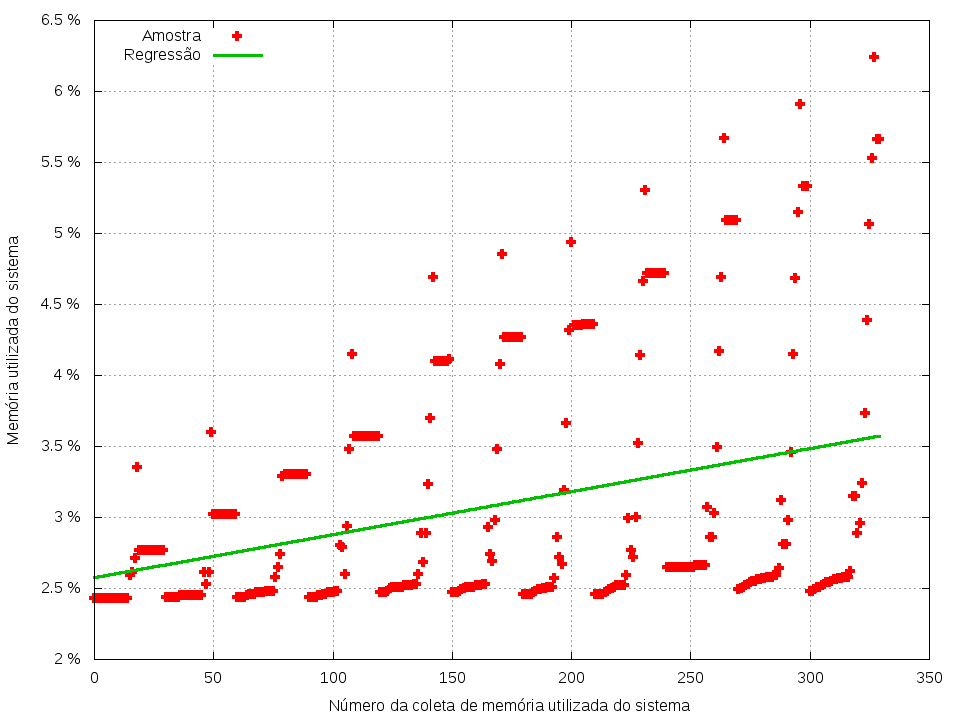
\includegraphics[scale=.35]{images/scatter-memory-usage}
    \end{figure}
\end{frame}


\begin{frame}{Taxa de escrita em memória secundária}

    \begin{figure}[!htb]
        \centering
        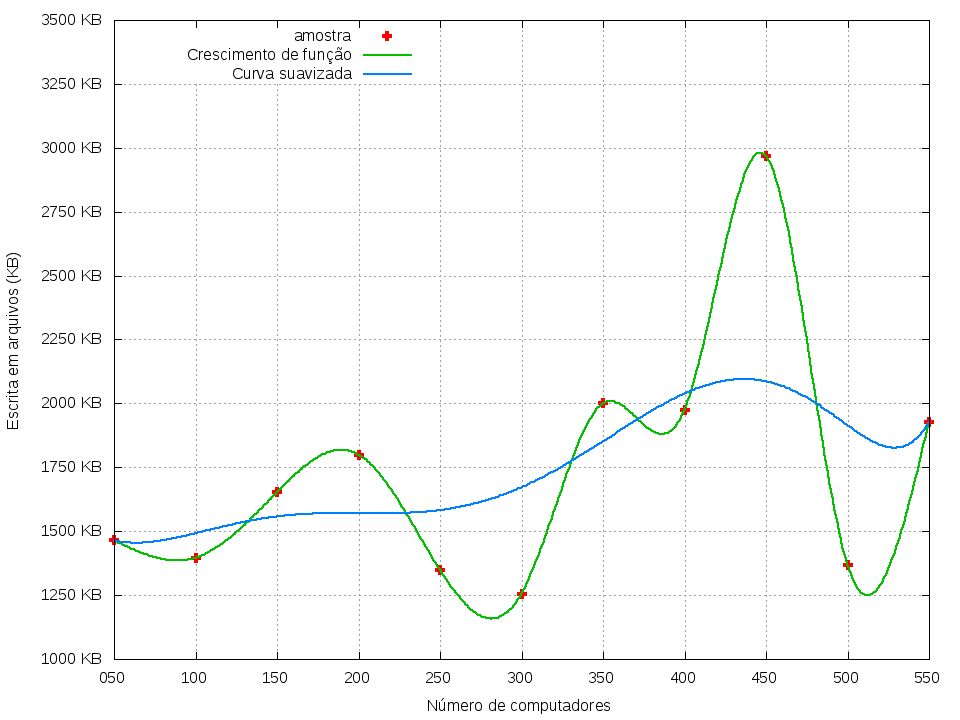
\includegraphics[scale=.35]{images/writing-rate-growth}
    \end{figure}
\end{frame}



\begin{frame}{Taxa de escrita em memória secundária}

    \begin{figure}[!htb]
        \centering
        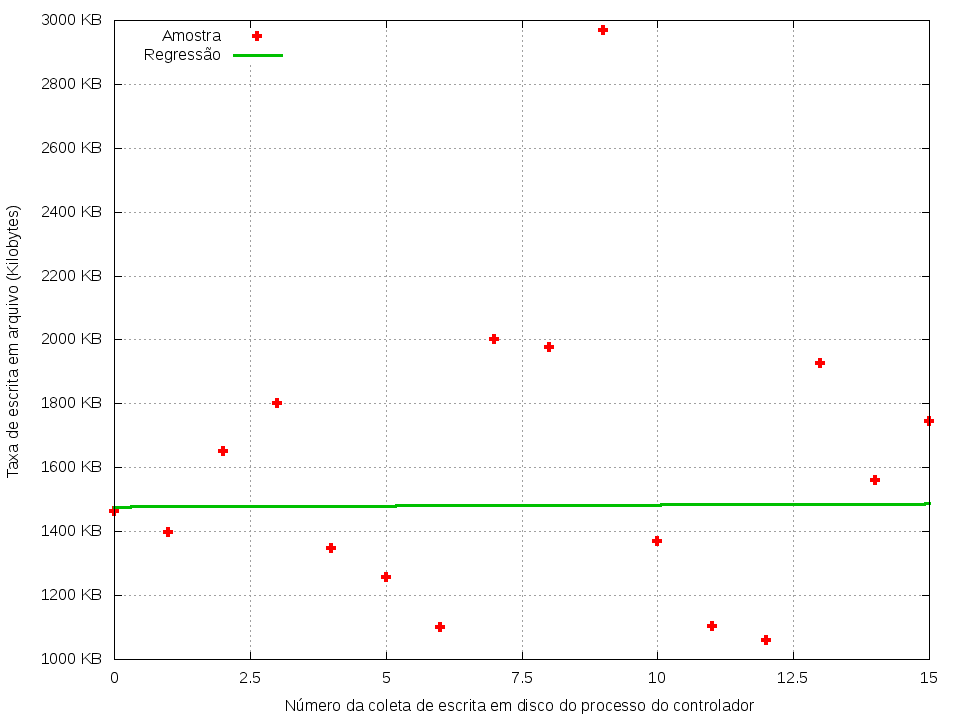
\includegraphics[scale=.35]{images/scatter-writing-rate}
    \end{figure}
\end{frame}


\begin{frame}{Avaliação do módulo \emph{host\_tracker}}
    
    \begin{table}[h!]
    \centering
    \begin{tabular}{ | l | l | l | l |}
    \hline
    \textbf{Teste} & \textbf{pingLim} & \textbf{entryMove} &
    \textbf{arpReply} \\ 
    \hline
    \hline Teste 0 & 5 & 50 & 5 \\ 
    \hline Teste 1 & 4 & 40 & 4 \\ 
    \hline Teste 2 & 3 & 30 & 3 \\ 
    \hline Teste 3 & 2 & 20 & 2 \\
    \hline Teste 4 & 1 & 10 & 1 \\
    \hline
    \end{tabular}
    \caption{Tabela com a relação de parâmetros por teste}
    \label{tbl:host_tracker-experiment}
\end{table}

\end{frame}


\begin{frame}{Largura de banda}

    \begin{figure}[!htb]
        \centering
        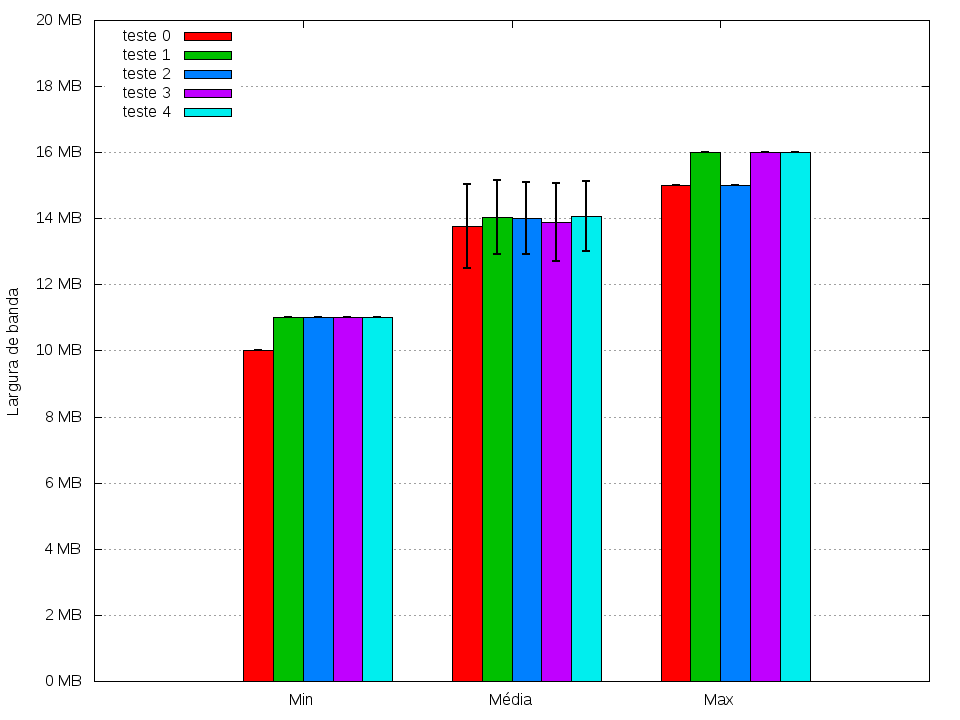
\includegraphics[scale=.35]{images/host_tracker-bandwidth}
    \end{figure}

\end{frame}


\begin{frame}{Interpolação da largura de banda}

    \begin{figure}[!htb]
        \centering
        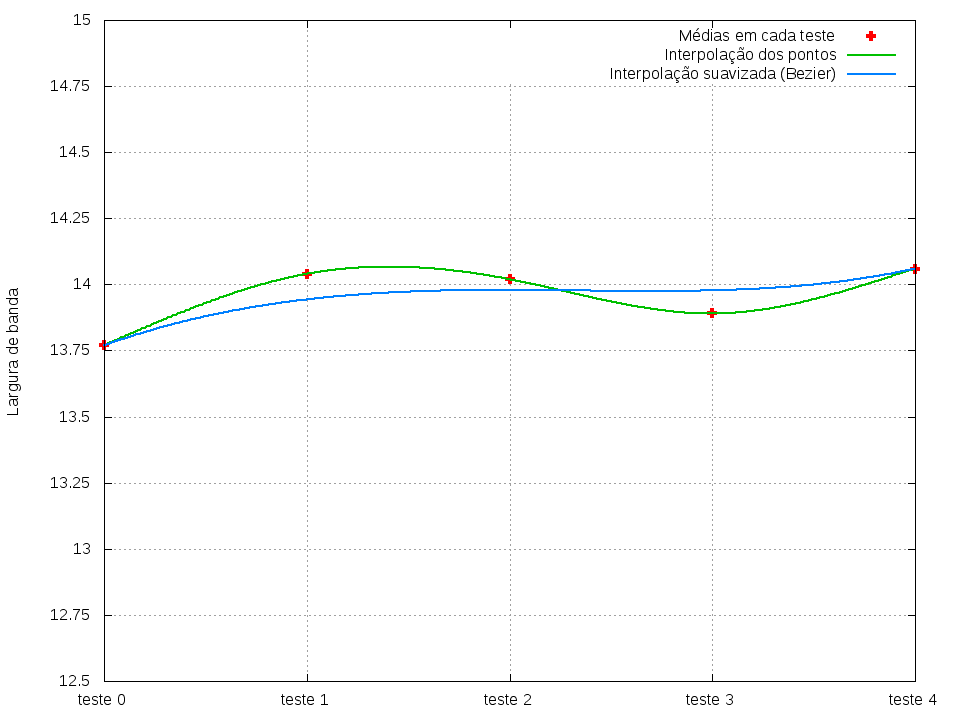
\includegraphics[scale=.35]{images/host_tracker-bandwidth-growth}
    \end{figure}

\end{frame}


\begin{frame}{Avaliação do número de pacotes}

    \begin{figure}[!htb]
        \centering
        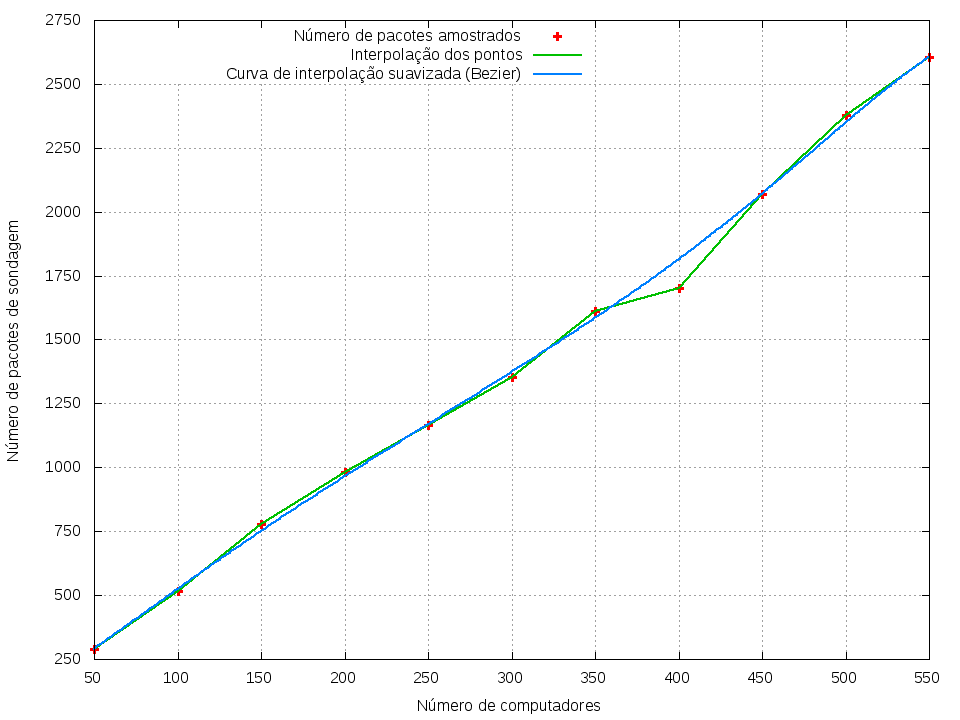
\includegraphics[scale=.35]{images/npings}
    \end{figure}
\end{frame}


\begin{frame}{Variação do número de pacotes na rede}

    \begin{figure}[!htb]
        \centering
        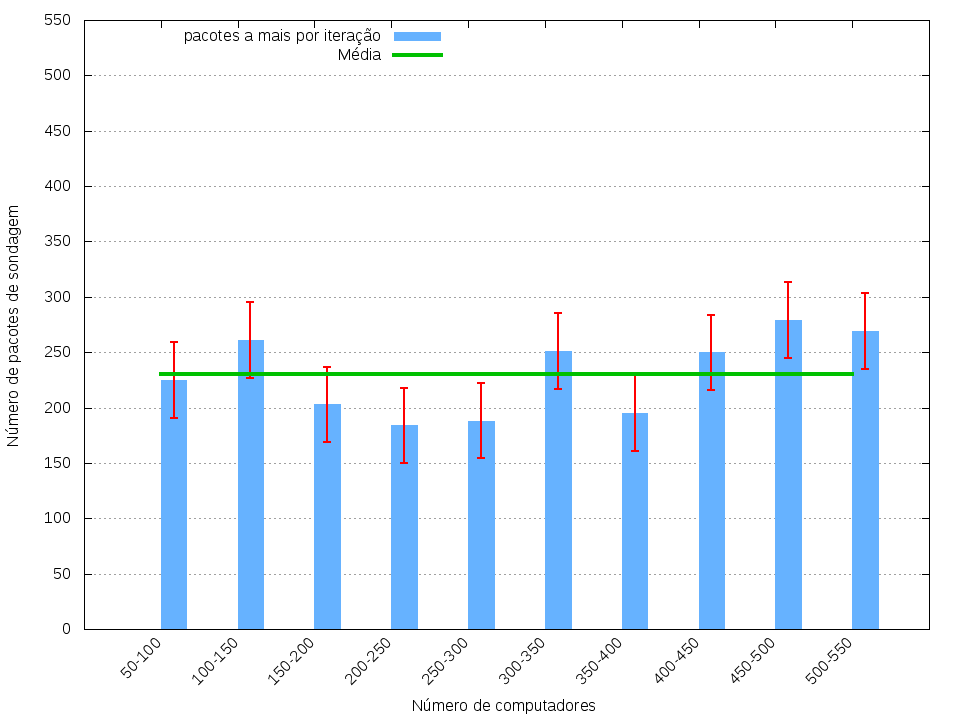
\includegraphics[scale=.35]{images/npings-stats}
    \end{figure}
\end{frame}


\begin{frame}{Variação do número de pacotes no controlador}

    \begin{figure}[!htb]
        \centering
        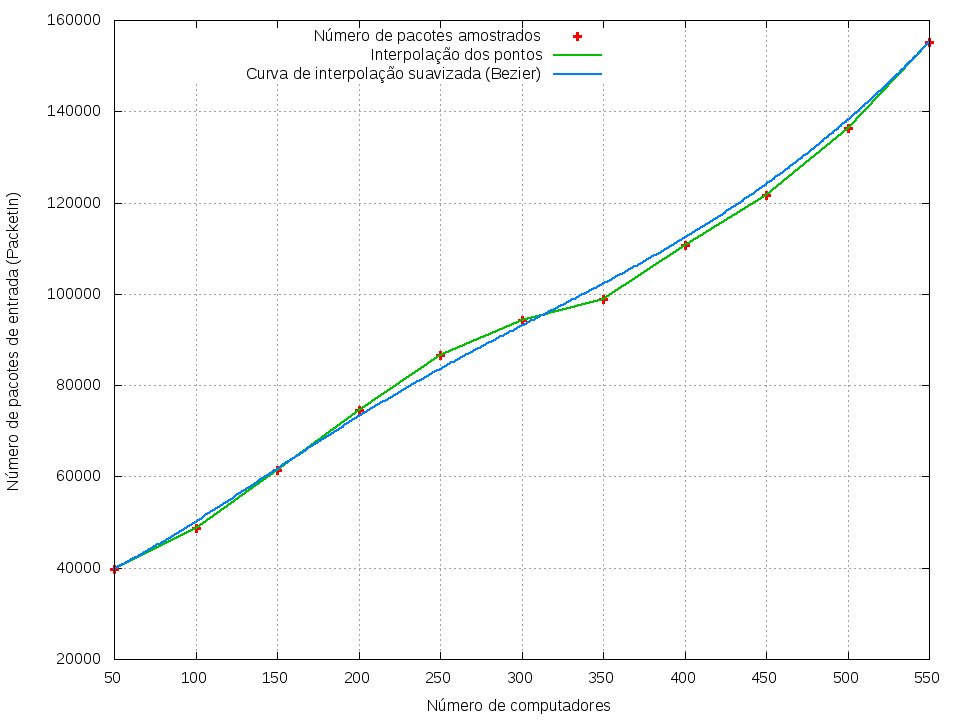
\includegraphics[scale=.35]{images/packets-in}
    \end{figure}
\end{frame}


\begin{frame}{Variação do número de pacotes no controlador}

    \begin{figure}[!htb]
        \centering
        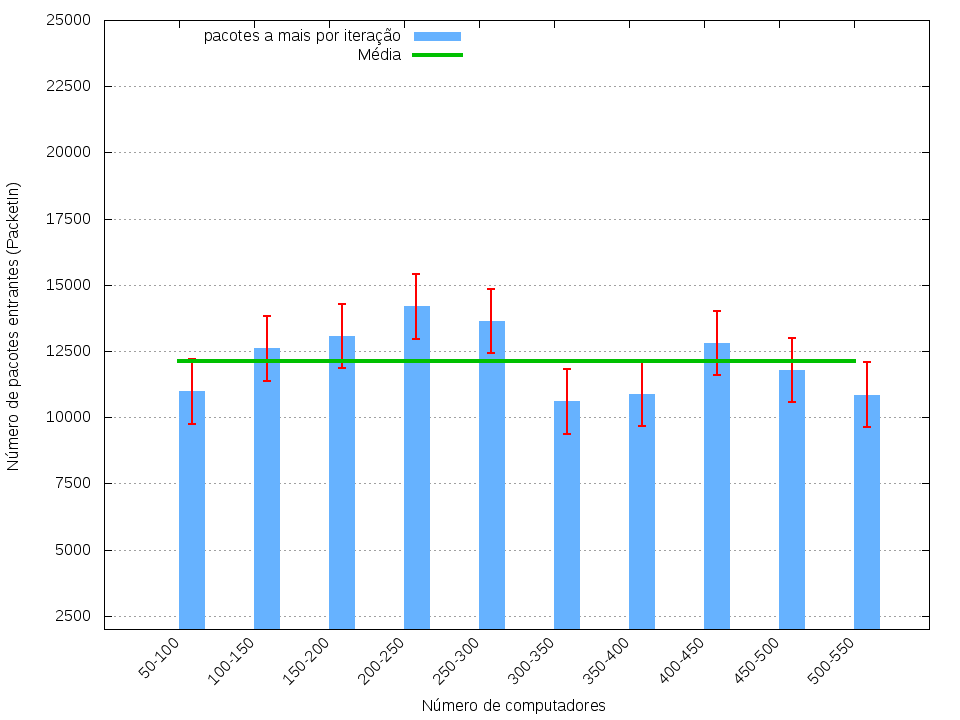
\includegraphics[scale=.35]{images/packets-in-stats}
    \end{figure}
\end{frame}


\begin{frame}{Comparação do número de pacotes}

    \begin{figure}[!htb]
        \centering
        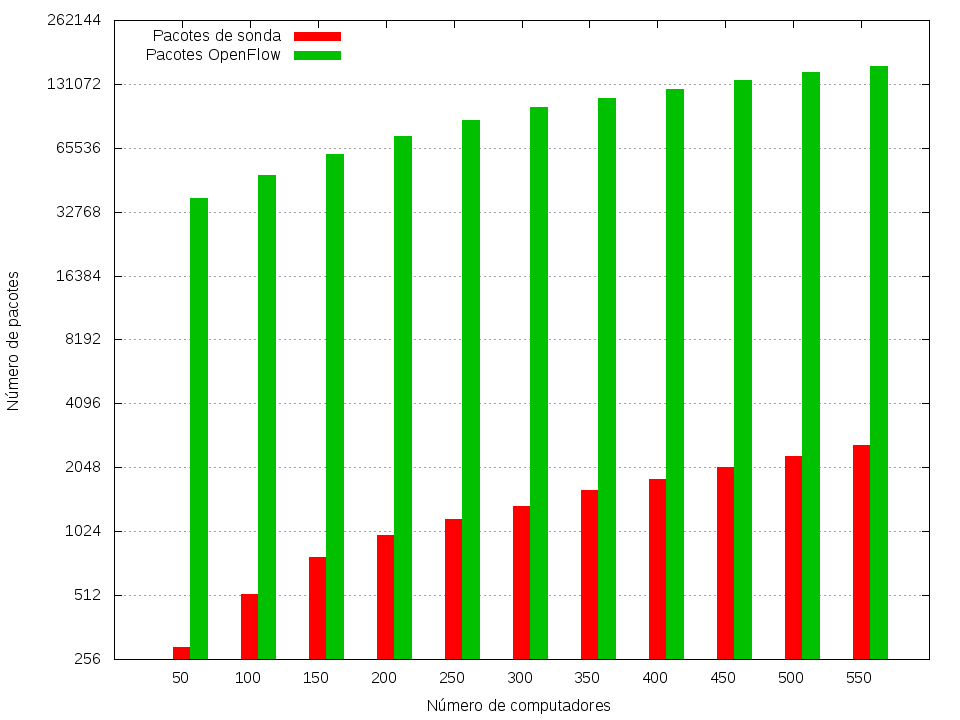
\includegraphics[scale=.35]{images/npings-x-packets-in}
    \end{figure}
\end{frame}


\begin{frame}{Comparação do percentual de pacotes}

    \begin{figure}[!htb]
        \centering
        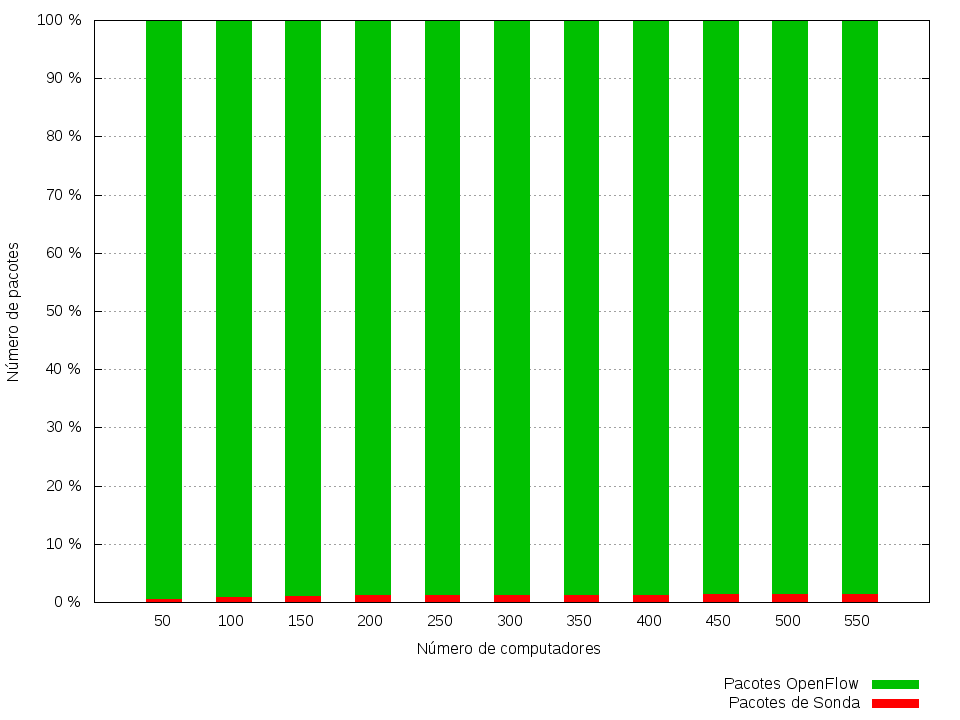
\includegraphics[scale=.35]{images/npings-x-packets-in-stacked}
    \end{figure}
\end{frame}



\begin{frame}{Avaliação da latência - rede local}

    \begin{figure}[!htb]
        \centering
        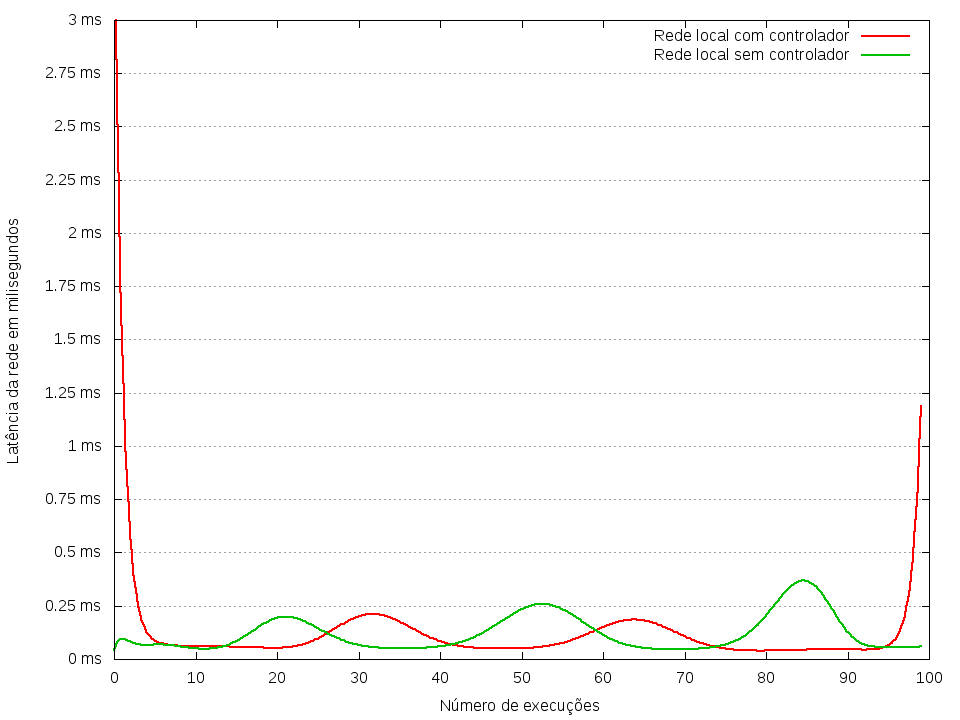
\includegraphics[scale=.35]{images/local-latency}
    \end{figure}
\end{frame}



\begin{frame}{Avaliação da latência - rede local}

    \begin{figure}[!htb]
        \centering
        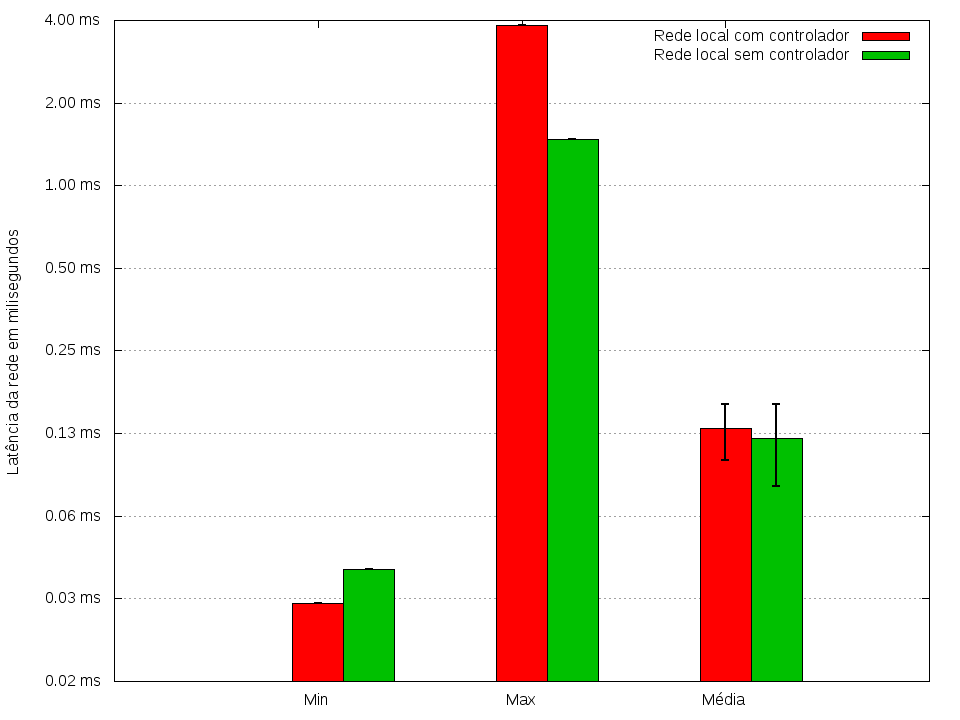
\includegraphics[scale=.35]{images/local-latency-stats}
    \end{figure}
\end{frame}


\begin{frame}{Avaliação da latência - rede Ipê}

    \begin{figure}[!htb]
        \centering
        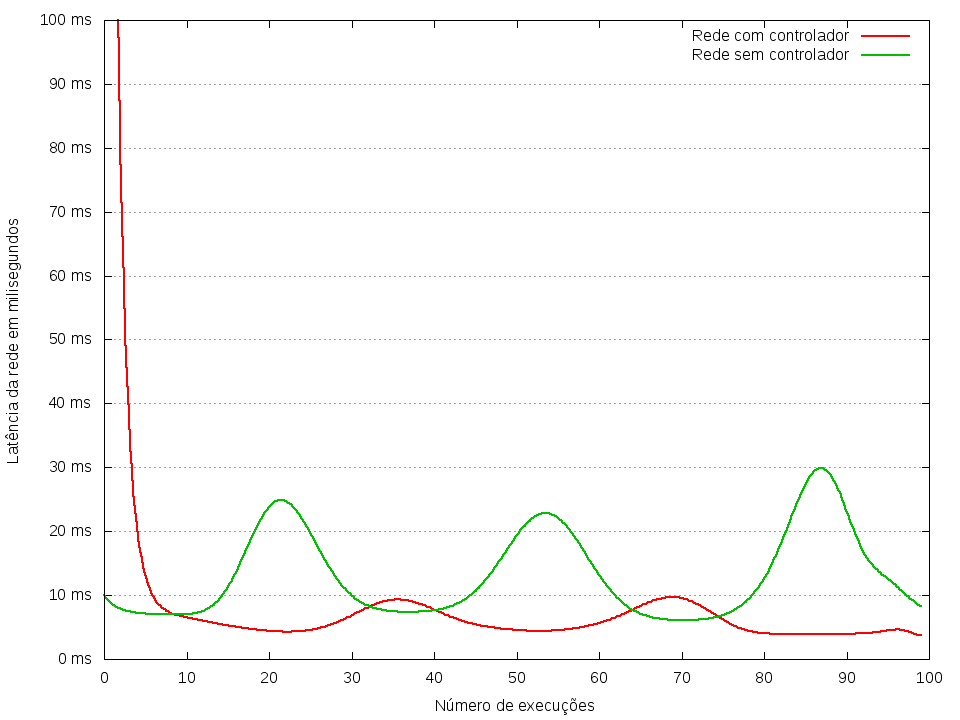
\includegraphics[scale=.35]{images/ipe-latency}
    \end{figure}
\end{frame}


\begin{frame}{Avaliação da latência - rede Ipê}

    \begin{figure}[!htb]
        \centering
        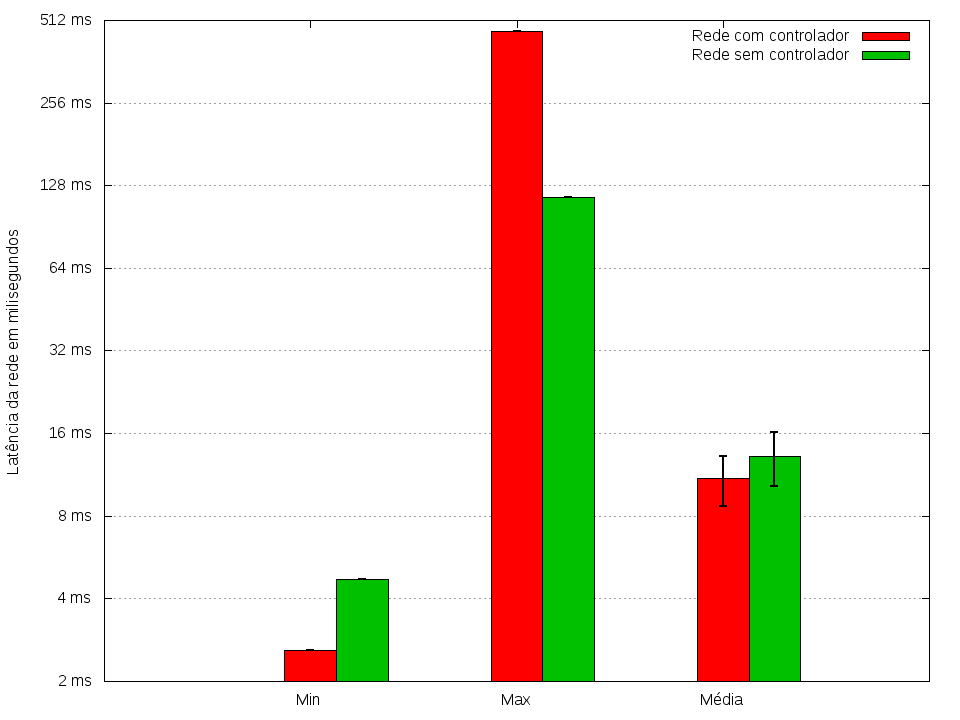
\includegraphics[scale=.35]{images/ipe-latency-stats}
    \end{figure}
\end{frame}


\begin{frame}{Avaliação da largura de banda sem controlador}

    \begin{figure}[!htb]
        \centering
        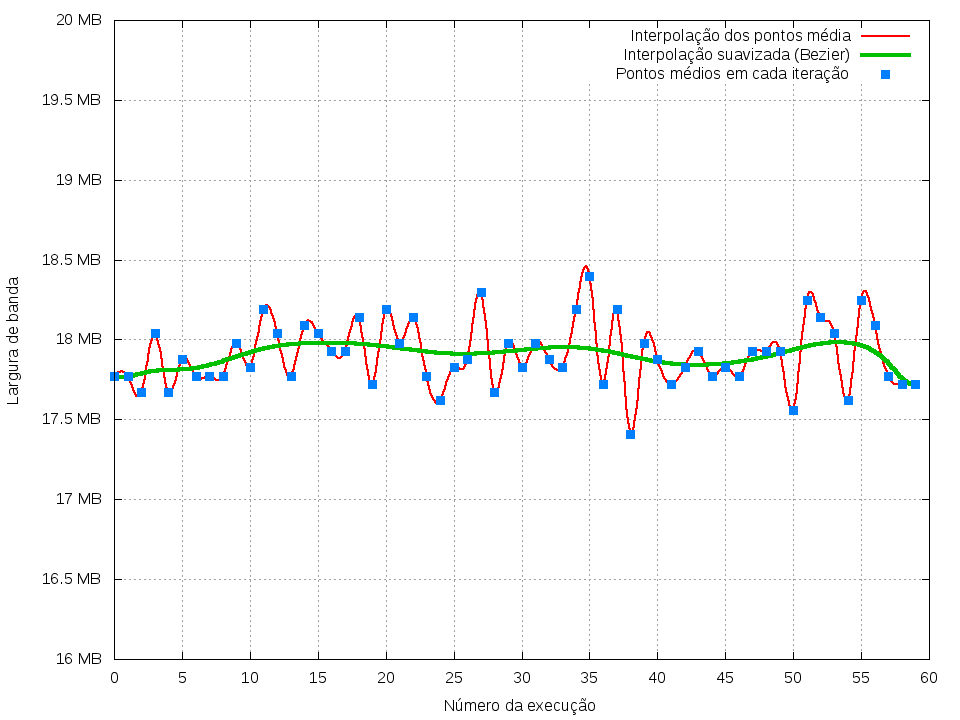
\includegraphics[scale=.35]{images/bandwidth-no-ctrl}
    \end{figure}
\end{frame}



\begin{frame}{Avaliação da largura de banda com controlador}

    \begin{figure}[!htb]
        \centering
        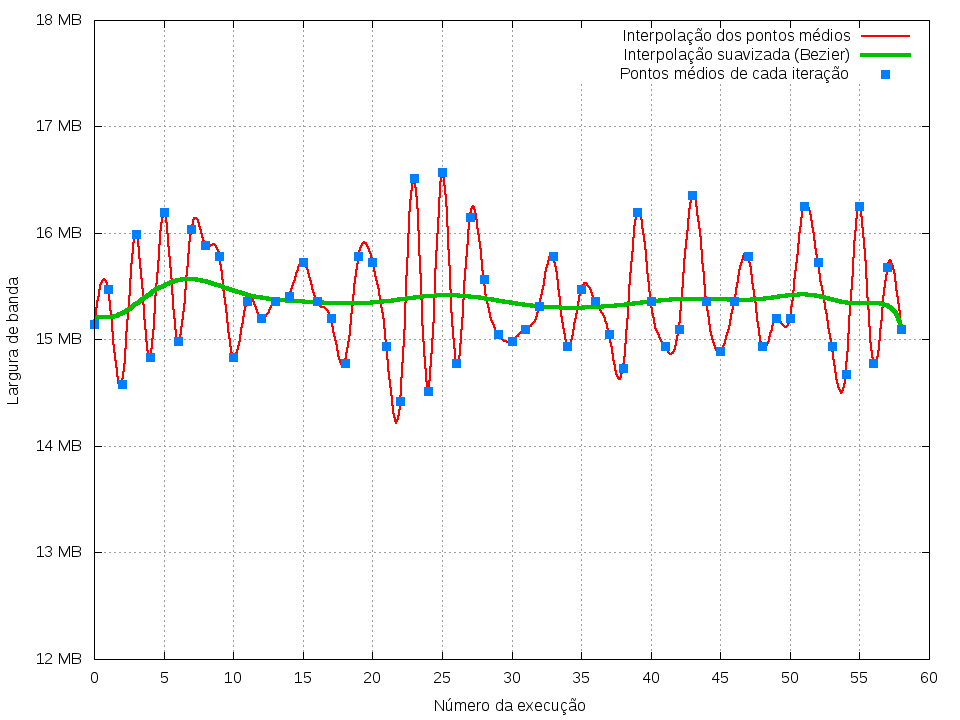
\includegraphics[scale=.35]{images/bandwidth-ctrl}
    \end{figure}
\end{frame}


\begin{frame}{Comparação da largura de banda}

    \begin{figure}[!htb]
        \centering
        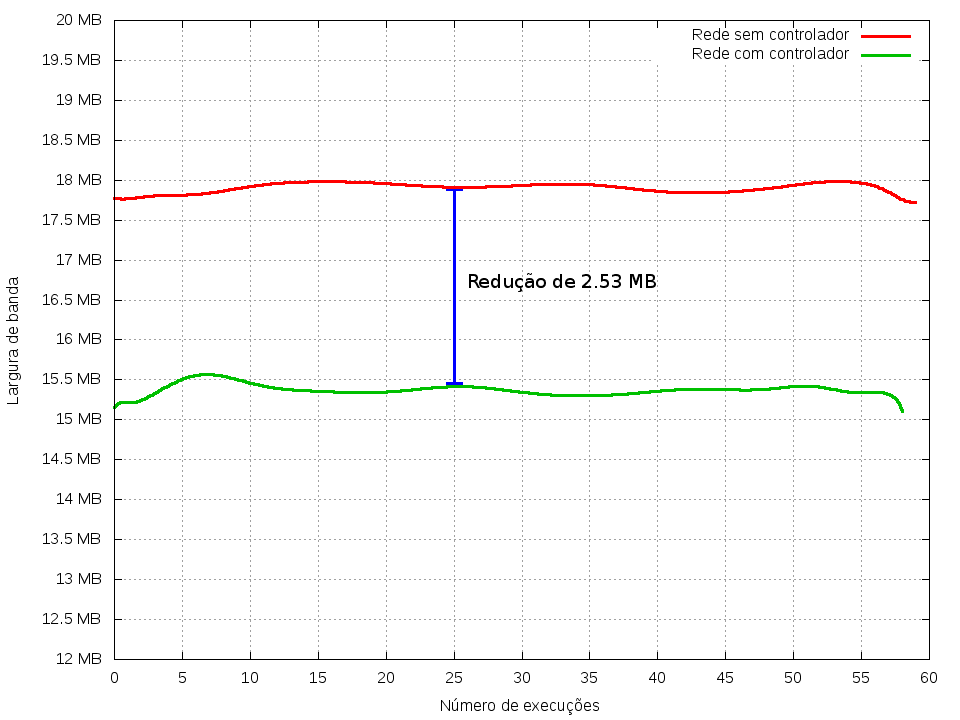
\includegraphics[scale=.35]{images/bandwidth-diff}
    \end{figure}
\end{frame}


\begin{frame}{Avaliação do \emph{Jitter} sem controlador}

    \begin{figure}[!htb]
        \centering
        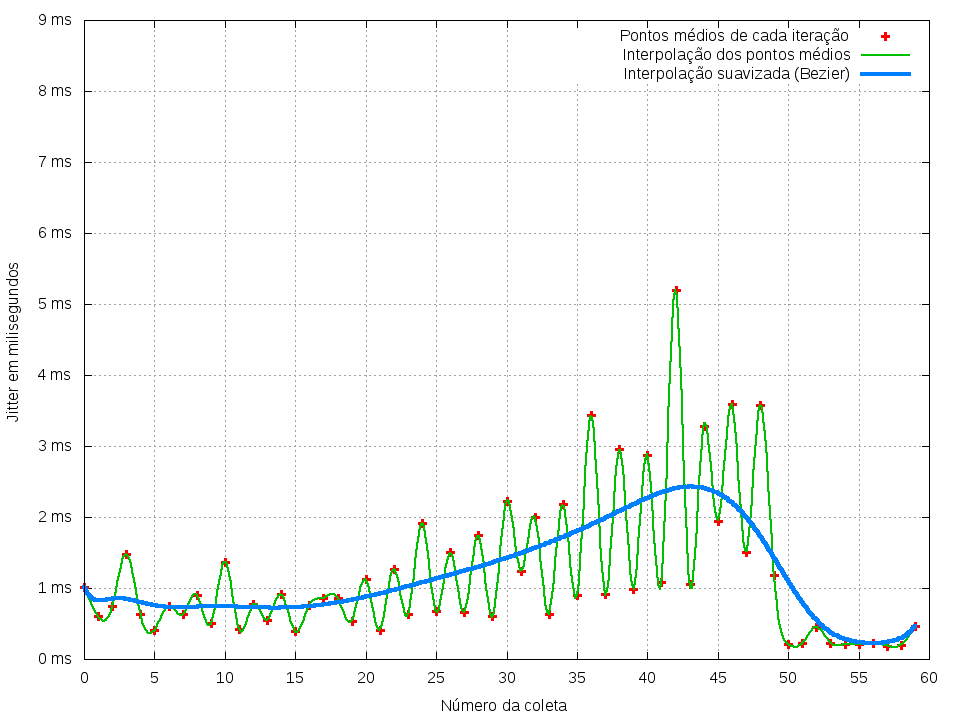
\includegraphics[scale=.35]{images/jitter-no-ctrl}
    \end{figure}
\end{frame}



\begin{frame}{Avaliação do \emph{Jitter} com controlador}

    \begin{figure}[!htb]
        \centering
        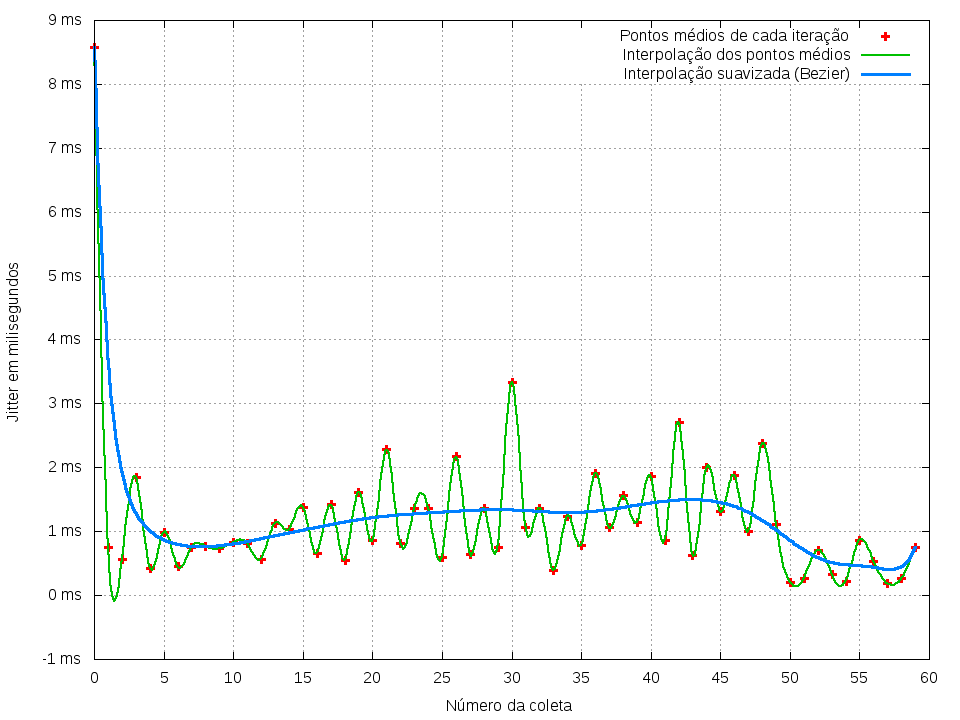
\includegraphics[scale=.35]{images/jitter-ctrl}
    \end{figure}
\end{frame}


\begin{frame}{Comparação do \emph{Jitter}}

    \begin{figure}[!htb]
        \centering
        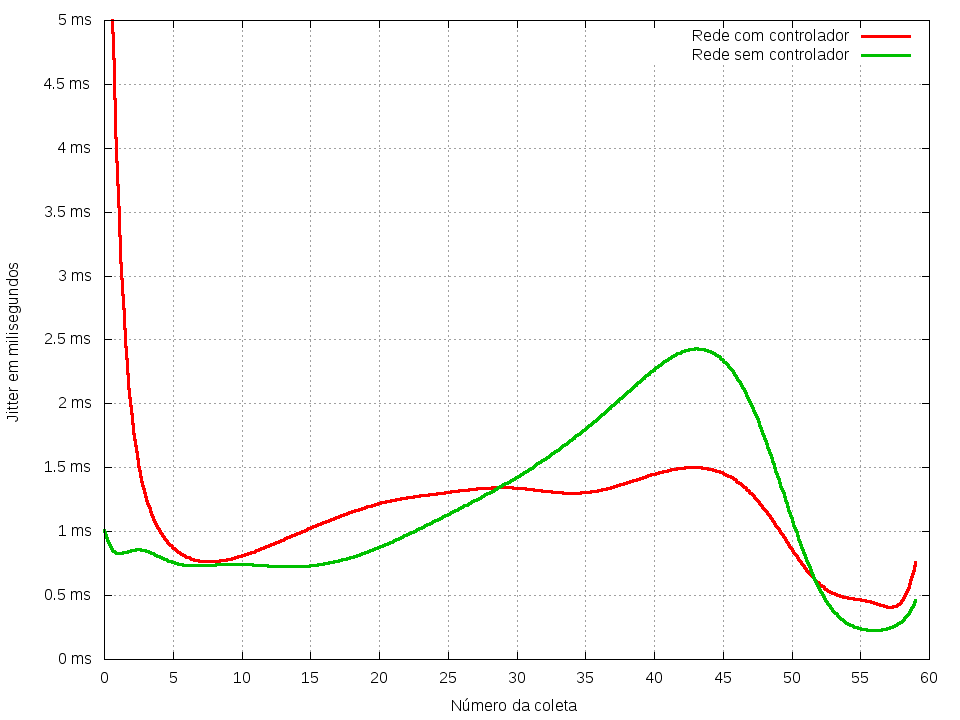
\includegraphics[scale=.35]{images/jitter-stats}
    \end{figure}
\end{frame}


\begin{frame}{Avaliação do percentual de erro}

    \begin{figure}[!htb]
        \centering
        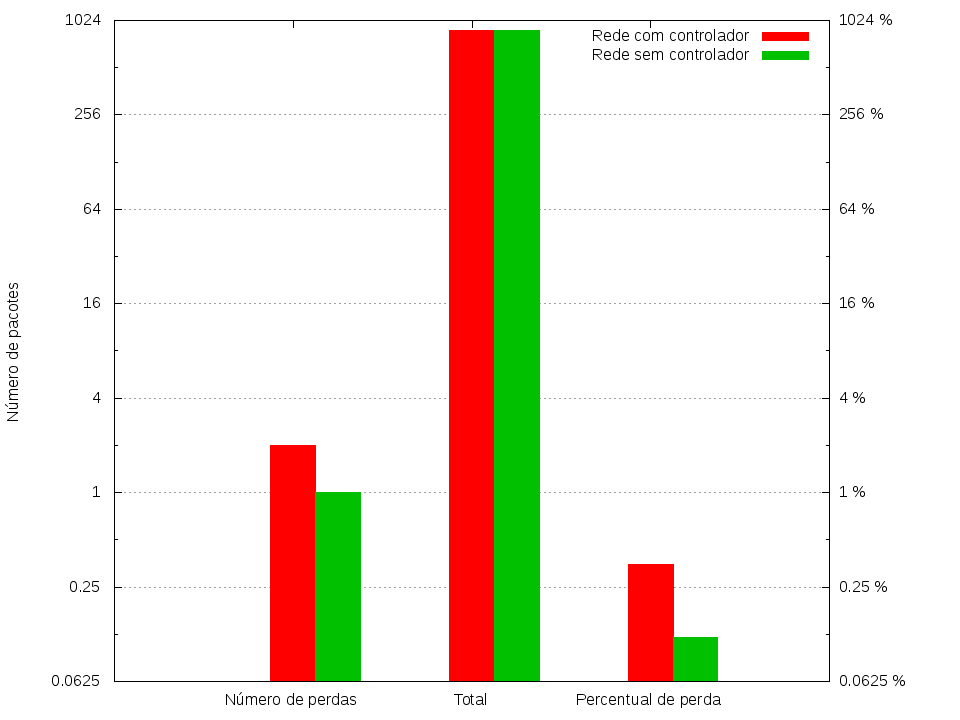
\includegraphics[scale=.35]{images/error-stats}
    \end{figure}
\end{frame}


